% ----------------------------------------------------------------------- %
% 						ITU Thesis LATEX Template						%
% 																		%
%							  UNOFFICIAL									%
% 							Version 2.0.0b								%
%						  by Mithat Can Özin								%
% ----------------------------------------------------------------------- %

% ---------------------------------------------------------------- %
% Prepared by ITU Informatics Institute	                           %
%                                                                  %
% Modified by Alican Mertan, Gülçin Baykal Can and Yusuf Özçevik   %
%                                                                  %
% Informatics Institute, ITU Ayazaga Campus                        %
% Maslak-34469, İstanbul, Turkey                                   %
% http://www.be.itu.edu.tr                                         %
% ---------------------------------------------------------------- %

% ----------------------------------------------------------------------- %
% Updated voluntarily by	  :												%
% Mithat Can Özin	:	ozin@itu.edu.tr									%
% E. Baris Ondes		:	ondes@itu.edu.tr		OR	ondesalt@pm.me			%
% Tamer Sener		:	senerta@itu.edu.tr	OR	senertam@pm.me			%
% Berkan Kacmaz		:	kacmazb@itu.edu.tr	OR	kacmazberkan0@gmail.com	%
% S. Baris Ozturk	:	ozturksb@itu.edu.tr	OR	salihbaris@gmail.com		%
% O. Ozgun Altunkaya	:	altunkayao@itu.edu.tr	OR	ozgun@pm.me 			%
% Latest update: 31-Dec-2024												%
% ----------------------------------------------------------------------- %

% ----------------------------------------------------------------------- %
% Please visit the following page for the current version:				%
% https://github.com/ondes/Template-Latex-ITU-Thesis						%
% ----------------------------------------------------------------------- %

% ----------------------------------------------------------------------- %
% 						DOCUMENT CLASS ARGUMENTS							%
% [onluarkali,tekyonlu], twoside/oneside									%                   
% [turkce,ingilizce], turkish/english									%
% [lisans,yukseklisans,doktora], BSc/MSc/PhD								%
% [bez,online], 	hardcover/online (Unofficial)							%
% [bilisim,lisansustu,sosyalbilimler,avrasya,enerji], institutes			%
% ----------------------------------------------------------------------  %
% Sample use:															%
% \documentclass[onluarkali,ingilizce,doktora,bez,lisansustu]{itutez}		%
% 																		%
% Other sample use:														% 
% \documentclass[tekyonlu,ingilizce,yukseklisans,online,bilisim]{itutez}  %
% 																		%
% ----------------------------------------------------------------------- %
% 						TANIMLAMALAR/DEFINITIONS					      	%
% onluarkali: twoside                     			  			 	  	%
% tekyonlu: oneside						 						 	  	%
% turkce: turkish							 						   	%
% ingilizce: english												   	    %
% lisans: undergraduate													%
% yukseklisans: masters												   	%
% doktora: phd								  						   	%
% bez: hardcover					  								        %
% online: online	(unofficial)			 			 				        %
% 						INSTITUES (For grad students)					%
% bilisim: informatics							  					    %
% lisansustu: graduate school										    %
% sosyalbilimler: social sciences					 				    %
% avrasya: eurasia						 								%
% enerji: energy															%
% 						FACULTIES (For undergrads)						%
% ucakuzay: aeronautics & astronautics 									%
% elektrikelektronik: electrical and electronics							%
% makina: mechanical engineering											%
% ---------------------------------------------------------------- %
\documentclass[onluarkali,ingilizce,yukseklisans,bez,lisansustu]{itutez}
% ----------------------------------------------------------------------- %
% 						USER PACKAGES (Optional)			          	  	% 
%-------------------------------------------------------------------------%

\usepackage{tikz} % tikz
% ----------------------------------------------------------------------- %
% 						USER DEFINITIONS (Optional)		                	%   
%-------------------------------------------------------------------------%

%-----------------------------%
% USER DEFINITIONS (OPTIONAL) %
%-----------------------------%

% Examples

% \def\be{\begin{equation}} %
% \def\ee{\end{equation}}%
% \def\beq{\begin{eqnarray}}%
% \def\eeq{\end{eqnarray}}%
% \def\bse{\begin{subequations}}%
% \def\ese{\end{subequations}}%
% \def\nonu{\nonumber}%
% \def\psibar{\overline{\psi}} %
% \def\Delslash{\partial\!\!\!\!\!/}%
% \def\Gslash{G\!\!\!\!\!/}%
% \def\Lmbdslash{\lambda\!\!\!\!\!/}%
% \def\Jslash{J\!\!\!\!\!/}%
% \def\pslash{p\!\!\!\!/}%
% \def\qslash{q\!\!\!\!/}%
% \def\kslash{k\!\!\!\!/}%
% \def\[{\left[}
% \def\]{\right]}
% \def\({\left(}
% \def\){\right)}

% \def\Lag{{\cal L}}    % 
% \def\D{{\cal D}}      % 
% \def\H{{\cal H}}      % 
% \def\Z{{\cal Z}}      % 
% \def\S{{\textbf{S}}}  % 
% \def\d{{\rm d}}%
% \def\dt{{\rm{dt}}}%
% \def\Tr{{\rm{Tr}}}%
% \def\gm{\gamma^{\mu}}
% \def\ga{\gamma^{\alpha}}
% \def\gb{\gamma^{\beta}}
% \def\gn{\gamma^{\nu}}
% \def\gs{\gamma^{\sigma}}
% \def\gl{\gamma^{\lambda}}
% \def\gr{\gamma^{\rho}}
% \def\gd{\gamma^{\delta}}




% ---------------------------------------------------------------- %
% Pay attention to letter case. The structure is case sensitive    %
% {Name}{SURNAME} means first letter of name is capital and that   %
% all letters of surname are capital.                              %
% ---------------------------------------------------------------- %

% ---------------------------------------------------------------- %
% No titles, only Name and SURNAME must be written.      	   %
% ---------------------------------------------------------------- %
\yazar{Name}{SURNAME} 
\ogrencino{702082003}

% ---------------------------------------------------------------- %
% If you do not use the structure, do not delete it. Just delete   %
% the argument. \unvan{} means title.                              %
% ---------------------------------------------------------------- %
\unvan{(Any Profession)}
 
% ---------------------------------------------------------------- %
% For below, the first argument for Turkish, the second is for     %
% English.       						   %
% ---------------------------------------------------------------- %

% ---------------------------------------------------------------- %
% Only the first letters of words must be capital.		   %
% ---------------------------------------------------------------- %
\anabilimdali{İnşaat Mühendisliği Anabilim Dalı}{Department of Civil Engineering}
\program{Yapı Mühendisliği Programı}{Structure Engineering Programme}

% ---------------------------------------------------------------- %
% For paperback version, the submission date to the faculty. For   %
% hardcover (indigo/black) version, date of defense.		   %
% ---------------------------------------------------------------- %

\tarih{TEZİN SAVUNULDUĞU AY YIL}{MONTH YEAR OF DEFENSE}
\tarihKucuk{Tezin savunulduğu ay yıl}{Month year of defense}

% ---------------------------------------------------------------- %
% Thesis advisor, title, thesis submission date, defense date      %
% ---------------------------------------------------------------- %
\danisman{Doç. Dr. Name SURNAME}{İstanbul Teknik Üniversitesi}   

\advisor{Assoc. Prof. Dr. Name SURNAME}{Istanbul Technical University}   


\baslik{TEZ BAŞLIĞI BURAYA GELİR}{GEREKLİ İSE İKİNCİ SATIR}{GEREKİ İSE ÜÇÜNCÜ SATIR,
ÜÇ SATIRA SIĞDIRINIZ}

\title{THESIS TITLE HERE}{SECOND LINE IF NECESSARY}{THIRD LINE IF NECESSARY, FIT TITLE IN THREE LINES}

% ---------------------------------------------------------------- %
% The date of submission of the paperback to the department.	   %
% ---------------------------------------------------------------- %
\tezvermetarih{22 Eylül 2009}{22 September 2009} 

\tezsavunmatarih{21 Aralık 2009}{21 December 2009}

% ---------------------------------------------------------------- %
% coadvisor and jury information. If you do not use all items,     %
% leave the corresponding arguments blank such as                  %
% \esdanismani{}{} 					           %
% ---------------------------------------------------------------- %
%\esdanisman{Dr. Öğretim Üyesi Name SURNAME}{İstanbul Teknik Üniversitesi}    
\esdanisman{}{}    

%\coadvisor{Assist. Prof. Dr. Name SURNAME}{Istanbul Technical University}   
\coadvisor{}{} 

\juriBir{Prof. Dr. Name SURNAME}{Yıldız Technical University}

\juriIki{Prof. Dr. Name SURNAME}{Boğaziçi University}

\juriUc{Prof. Dr. Name SURNAME}{Gebze Institute of Technology}

\juriDort{Prof. Dr. Name SURNAME}{Şişli Etfal Teaching Hospital}

\juriBes{Prof. Dr. Name SURNAME}{Bilkent University}

% ---------------------------------------------------------------- %
% For dedication page. Leave the argument blank if not used.	   %
% ---------------------------------------------------------------- %
\ithaf{To my spouse and children,}

% ---------------------------------------------------------------- %
% Form the below files						   %
% ---------------------------------------------------------------- %
\onsoz{For the foreword, 1 line spacing must be set. The foreword, written
as a first page of the thesis must not exceed 2 pages. The 
acknowledgements must be given in this section.
After the foreword text, name of the author (right-aligned), and
the date (as month and year) must be written (left-aligned). Surnames should be capitalized. These two expressions must be in the same line. The foreword is written with 1 line spacing.}
\kisaltmalistesi{\renewcommand{\arraystretch}{1.5}
\begin{tabular}{@{}p{2cm}l}
{\bf{AIC}} & {\bf:} Akaike Information Criteria\\
{\bf ANN} & {\bf:} Artificial Neural Network\\
{\bf App} & {\bf:} Appendix\\
{\bf BP} & {\bf:} Backpropagation\\
{\bf CGI} & {\bf:} Common Gateway Interface\\
{\bf ESS} & {\bf:} Error sum-of-squares\\
{\bf GARCH} & {\bf:} Generalized Autoregressive Conditional Heteroskedasticity\\
{\bf GIS} & {\bf:} Geographic Information Systems\\
{\bf HCA} & {\bf:} Hierarchical Cluster Analysis\\
{\bf Mbps} & {\bf:} Megabits\\
{\bf St} & {\bf:} Station\\
{\bf SWAT} & {\bf:} Soil and Water Assessment Tool\\
{\bf UMN} & {\bf:} University of Minnesota\\
\end{tabular}
\renewcommand{\arraystretch}{1.0}
}
\sembollistesi{
\begin{tabular}{p{2cm}l}
{\bf{C}} & {\bf:} Capacitance\\
{\bf H} & {\bf:} The amount of heat\\
{\bf M\textsubscript{x},} {\bf M\textsubscript{y}} & {\bf:} Torque Components\\
{\bf N\textsubscript{x},} {\bf N\textsubscript{y},} {\bf N\textsubscript{z}} & {\bf:} Normal Power Components\\
{\bf q} & {\bf:} Phase load\\
{\bf t} & {\bf:} Time\\
{\bf u, v} & {\bf:} Displacement Vector Components\\
{\bf w} & {\bf:} Angular velocity\\
{\bf XC} & {\bf:} Capacitive reactance\\
{\bf XL} & {\bf:}  Inductive reactance\\
%{\bf {\textalpha}} & {\bf:} Asal gerilme do\u{g}rultusundan sapma a\c{c}\i s\i\\
%{\bf {\textrho}} & {\bf:} Yo\u{g}unluk\\
%{\bf {\textsigma\textsubscript{x},}} {\bf {\textsigma\textsubscript{y},}} {\bf {\textsigma\textsubscript{xy}}} & {\bf:} Kabuk i\c{c} gerilmeleri\\
\end{tabular}

}
\ozet{1 line spacing must be set for summaries. For theses in Turkish, the summary in Turkish must have 300 words minimum and span 1 to 3 pages, whereas the extended summary in English must span 3-5 pages.

For theses in English, the summary in English must have 300 words minimum and span 1-3 pages, whereas the extended summary in Turkish must span 3-5 pages.

A summary must briefly mention the subject of the thesis, the method(s) used and the conclusions derived.

References, figures and tables must not be given in Summary.

Above the Summary, the thesis title in first level title format (i.e., 72 pt before and 18 pt after paragraph spacing, and 1 line spacing) must be placed. Below the title, the expression ÖZET (for summary in Turkish) and SUMMARY (for summary in English) must be written horizontally centered.

It is recommended that the summary in English is placed before the summary in Turkish.
Lorem ipsum dolor sit amet, consetetur sadipscing elitr, sed diam nonumy eirmod tempor invidunt ut labore et dolore magna aliquyam erat, sed diam voluptua. At vero eos et accusam et justo duo dolores et ea rebum. Stet clita kasd gub rgren, no sea takimata sanctus est Lorem ipsum dolor sit amet, consetetur sadipscing elitr, sed diam nonumy eirmod tempor invidunt ut lab ore sit et dolore magna.

Lorem ipsum dolor sit amet, consetetur sadipscing elitr, sed diam nonumy eirmod tempor invidunt ut labore et dolore magna aliquyam erat, sed diam voluptua. At vero eos et accusam et justo duo dolores et ea rebum. Stet clita kasd gub rgren, no sea takimata sanctus est Lorem ipsum dolor sit amet, consetetur sadipscing elitr, sed diam nonumy eirmod tempor invidunt ut lab ore sit et dolore magna.

Lorem ipsum dolor sit amet, consetetur sadipscing elitr, sed diam nonumy eirmod tempor invidunt ut labore et dolore magna aliquyam erat, sed diam voluptua. At vero eos et accusam et justo duo dolores et ea rebum. Stet clita kasd gub rgren, no sea takimata sanctus est Lorem ipsum dolor sit amet, consetetur sadipscing elitr, sed diam nonumy eirmod tempor invidunt ut lab ore sit et dolore magna.

Lorem ipsum dolor sit amet, consetetur sadipscing elitr, sed diam nonumy eirmod tempor invidunt ut labore et dolore magna aliquyam erat, sed diam voluptua. At vero eos et accusam et justo duo dolores et ea rebum. Stet clita kasd gub rgren, no sea takimata sanctus est Lorem ipsum dolor sit amet, consetetur sadipscing elitr, sed diam nonumy eirmod tempor invidunt ut lab ore sit et dolore magna.

Lorem ipsum dolor sit amet, consetetur sadipscing elitr, sed diam nonumy eirmod tempor invidunt ut labore et dolore magna aliquyam erat, sed diam voluptua. At vero eos et accusam et justo duo dolores et ea rebum. Stet clita kasd gub rgren, no sea takimata sanctus est Lorem ipsum dolor sit amet, consetetur sadipscing elitr, sed diam nonumy eirmod tempor invidunt ut lab ore sit et dolore magna.

Lorem ipsum dolor sit amet, consetetur sadipscing elitr, sed diam nonumy eirmod tempor invidunt ut labore et dolore magna aliquyam erat, sed diam voluptua. At vero eos et accusam et justo duo dolores et ea rebum. Stet clita kasd gub rgren, no sea takimata sanctus est Lorem ipsum dolor sit amet, consetetur sadipscing elitr, sed diam nonumy eirmod tempor invidunt ut lab ore sit et dolore magna.

Lorem ipsum dolor sit amet, consetetur sadipscing elitr, sed diam nonumy eirmod tempor invidunt ut labore et dolore magna aliquyam erat, sed diam voluptua. At vero eos et accusam et justo duo dolores et ea rebum. Stet clita kasd gub rgren, no sea takimata sanctus est Lorem ipsum dolor sit amet, consetetur sadipscing elitr, sed diam nonumy eirmod tempor invidunt ut lab ore sit et dolore magna.

Lorem ipsum dolor sit amet, consetetur sadipscing elitr, sed diam nonumy eirmod tempor invidunt ut labore et dolore magna aliquyam erat, sed diam voluptua. At vero eos et accusam et justo duo dolores et ea rebum. Stet clita kasd gub rgren, no sea takimata sanctus est Lorem ipsum dolor sit amet, consetetur sadipscing elitr, sed diam nonumy eirmod tempor invidunt ut lab ore sit et dolore magna.

Lorem ipsum dolor sit amet, consetetur sadipscing elitr, sed diam nonumy eirmod tempor invidunt ut labore et dolore magna aliquyam erat, sed diam voluptua. At vero eos et accusam et justo duo dolores et ea rebum. Stet clita kasd gub rgren, no sea takimata sanctus est Lorem ipsum dolor sit amet, consetetur sadipscing elitr, sed diam nonumy eirmod tempor invidunt ut lab ore sit et dolore magna.

Lorem ipsum dolor sit amet, consetetur sadipscing elitr, sed diam nonumy eirmod tempor invidunt ut labore et dolore magna aliquyam erat, sed diam voluptua. At vero eos et accusam et justo duo dolores et ea rebum. Stet clita kasd gub rgren, no sea takimata sanctus est Lorem ipsum dolor sit amet, consetetur sadipscing elitr, sed diam nonumy eirmod tempor invidunt ut lab ore sit et dolore magna.

Lorem ipsum dolor sit amet, consetetur sadipscing elitr, sed diam nonumy eirmod tempor invidunt ut labore et dolore magna aliquyam erat, sed diam voluptua. At vero eos et accusam et justo duo dolores et ea rebum. Stet clita kasd gub rgren, no sea takimata sanctus est Lorem ipsum dolor sit amet, consetetur sadipscing elitr, sed diam nonumy eirmod tempor invidunt ut lab ore sit et dolore magna.

Lorem ipsum dolor sit amet, consetetur sadipscing elitr, sed diam nonumy eirmod tempor invidunt ut labore et dolore magna aliquyam erat, sed diam voluptua. At vero eos et accusam et justo duo dolores et ea rebum. Stet clita kasd gub rgren, no sea takimata sanctus est Lorem ipsum dolor sit amet, consetetur sadipscing elitr, sed diam nonumy eirmod tempor invidunt ut lab ore sit et dolore magna.

Lorem ipsum dolor sit amet, consetetur sadipscing elitr, sed diam nonumy eirmod tempor invidunt ut labore et dolore magna aliquyam erat, sed diam voluptua. At vero eos et accusam et justo duo dolores et ea rebum. Stet clita kasd gub rgren, no sea takimata sanctus est Lorem ipsum dolor sit amet, consetetur sadipscing elitr, sed diam nonumy eirmod tempor invidunt ut lab ore sit et dolore magna.

Lorem ipsum dolor sit amet, consetetur sadipscing elitr, sed diam nonumy eirmod tempor invidunt ut labore et dolore magna aliquyam erat, sed diam voluptua. At vero eos et accusam et justo duo dolores et ea rebum. Stet clita kasd gub rgren, no sea takimata sanctus est Lorem ipsum dolor sit amet, consetetur sadipscing elitr, sed diam nonumy eirmod tempor invidunt ut lab ore sit et dolore magna.

Lorem ipsum dolor sit amet, consetetur sadipscing elitr, sed diam nonumy eirmod tempor invidunt ut labore et dolore magna aliquyam erat, sed diam voluptua. At vero eos et accusam et justo duo dolores et ea rebum. Stet clita kasd gub rgren, no sea takimata sanctus est Lorem ipsum dolor sit amet, consetetur sadipscing elitr, sed diam nonumy eirmod tempor invidunt ut lab ore sit et dolore magna.

Lorem ipsum dolor sit amet, consetetur sadipscing elitr, sed diam nonumy eirmod tempor invidunt ut labore et dolore magna aliquyam erat, sed diam voluptua. At vero eos et accusam et justo duo dolores et ea rebum. Stet clita kasd gub rgren, no sea takimata sanctus est Lorem ipsum dolor sit amet, consetetur sadipscing elitr, sed diam nonumy eirmod tempor invidunt ut lab ore sit et dolore magna.

Lorem ipsum dolor sit amet, consetetur sadipscing elitr, sed diam nonumy eirmod tempor invidunt ut labore et dolore magna aliquyam erat, sed diam voluptua. At vero eos et accusam et justo duo dolores et ea rebum. Stet clita kasd gub rgren, no sea takimata sanctus est Lorem ipsum dolor sit amet, consetetur sadipscing elitr, sed diam nonumy eirmod tempor invidunt ut lab ore sit et dolore magna.

Lorem ipsum dolor sit amet, consetetur sadipscing elitr, sed diam nonumy eirmod tempor invidunt ut labore et dolore magna aliquyam erat, sed diam voluptua. At vero eos et accusam et justo duo dolores et ea rebum. Stet clita kasd gub rgren, no sea takimata sanctus est Lorem ipsum dolor sit amet, consetetur sadipscing elitr, sed diam nonumy eirmod tempor invidunt ut lab ore sit et dolore magna.

Lorem ipsum dolor sit amet, consetetur sadipscing elitr, sed diam nonumy eirmod tempor invidunt ut labore et dolore magna aliquyam erat, sed diam voluptua. At vero eos et accusam et justo duo dolores et ea rebum. Stet clita kasd gub rgren, no sea takimata sanctus est Lorem ipsum dolor sit amet, consetetur sadipscing elitr, sed diam nonumy eirmod tempor invidunt ut lab ore sit et dolore magna.

Lorem ipsum dolor sit amet, consetetur sadipscing elitr, sed diam nonumy eirmod tempor invidunt ut labore et dolore magna aliquyam erat, sed diam voluptua. At vero eos et accusam et justo duo dolores et ea rebum. Stet clita kasd gub rgren, no sea takimata sanctus est Lorem ipsum dolor sit amet, consetetur sadipscing elitr, sed diam nonumy eirmod tempor invidunt ut lab ore sit et dolore magna.

Lorem ipsum dolor sit amet, consetetur sadipscing elitr, sed diam nonumy eirmod tempor invidunt ut labore et dolore magna aliquyam erat, sed diam voluptua. At vero eos et accusam et justo duo dolores et ea rebum. Stet clita kasd gub rgren, no sea takimata sanctus est Lorem ipsum dolor sit amet, consetetur sadipscing elitr, sed diam nonumy eirmod tempor invidunt ut lab ore sit et dolore magna.

Lorem ipsum dolor sit amet, consetetur sadipscing elitr, sed diam nonumy eirmod tempor invidunt ut labore et dolore magna aliquyam erat, sed diam voluptua. At vero eos et accusam et justo duo dolores et ea rebum. Stet clita kasd gub rgren, no sea takimata sanctus est Lorem ipsum dolor sit amet, consetetur sadipscing elitr, sed diam nonumy eirmod tempor invidunt ut lab ore sit et dolore magna.
}              
\summary{1 line spacing must be set for summaries. For theses in Turkish, the summary in
Turkish must have 300 words minimum and span 1 to 3 pages, whereas the extended
summary in English must span 3-5 pages.
For theses in English, the summary in English must have 300 words minimum and
span 1-3 pages, whereas the extended summary in Turkish must span 3-5 pages.
A summary must briefly mention the subject of the thesis, the method(s) used and 
the conclusions derived.
References, figures and tables must not be given in Summary.
Above the Summary, the thesis title in first level title format 
(i.e., 72 pt before and 18 pt after paragraph spacing, and 1 line 
spacing) must be placed. Below the title, expression {\bf \"OZET} 
(for summary in Turkish) and {\bf SUMMARY} (for summary in English)
must be written horizontally centered.
It is recommended that the summary in English is placed before
the summary in Turkish.

Lorem ipsum dolor sit amet, consectetur adipiscing elit. Praesent imperdiet, nisi 
nec aliquam cursus, dui turpis mollis nisl, ac consequat tellus sapien sit amet 
magna. Duis vel venenatis velit. Vestibulum ante ipsum primis in faucibus orci 
luctus et ultrices posuere cubilia Curae; Proin malesuada risus nec metus dapibus 
eu tincidunt lectus dignissim. Morbi massa orci, luctus at vulputate lacinia, 
vestibulum sed libero. Ut accumsan tortor vulputate dolor semper id dignissim 
augue semper. Proin ac purus mi. 

Lorem ipsum dolor sit amet, consectetur adipiscing elit. Praesent imperdiet, nisi 
nec aliquam cursus, dui turpis mollis nisl, ac consequat tellus sapien sit amet 
magna. Duis vel venenatis velit. Vestibulum ante ipsum primis in faucibus orci 
luctus et ultrices posuere cubilia Curae; Proin malesuada risus nec metus dapibus 
eu tincidunt lectus dignissim. Morbi massa orci, luctus at vulputate lacinia, 
vestibulum sed libero. Ut accumsan tortor vulputate dolor semper id dignissim 
augue semper. Proin ac purus mi. 

Lorem ipsum dolor sit amet, consectetur adipiscing elit. Praesent imperdiet, nisi 
nec aliquam cursus, dui turpis mollis nisl, ac consequat tellus sapien sit amet 
magna. Duis vel venenatis velit. Vestibulum ante ipsum primis in faucibus orci 
luctus et ultrices posuere cubilia Curae; Proin malesuada risus nec metus dapibus 
eu tincidunt lectus dignissim. Morbi massa orci, luctus at vulputate lacinia, 
vestibulum sed libero. Ut accumsan tortor vulputate dolor semper id dignissim 
augue semper. Proin ac purus mi. } 
\ozgecmis{\vspace{10mm}

%\newsavebox{\mysquare}
%\savebox{\mysquare}{\textcolor{black}{\rule[2.3pt]{3.4pt}{3.4pt}}}

%\setlength{\TPHorizModule}{10pt}
%\setlength{\TPVertModule}{10pt}
%\begin{textblock}{1}(40,10)
% \begin{figure}[p]
% 
\includegraphics[scale=0.3,keepaspectratio=true]{./fig/photo}
%\end{figure}
%\end{textblock}

\textbf{Name SURNAME:} \\

%\vspace{-3mm}
%\textbf{Place and Date of Birth:} \\

%\vspace{-3mm}
%\textbf{E-Mail:} \\


\textbf{EDUCATION:} 
\vspace{-3mm}
\begin{itemize}
  \item \textbf{B.Sc.:} Graduation year, University, Faculty, Department
  \item \textbf{M.Sc.:} Graduation year, University, Faculty, Department
\end{itemize}

\textbf{PROFESSIONAL EXPERIENCE AND REWARDS:}   
\vspace{-3mm}
\begin{itemize}
  \item 1950-1956 İstanbul Technical University at the Central Laboratory of Theoretical Physics.
  \item 1953 Nobel Prize for Physics
  \item 1956 Completed Doctorate at İstanbul Technical University
\end{itemize}

\textbf{PUBLICATIONS, PRESENTATIONS AND PATENTS ON THE THESIS:} 
\vspace{-3mm}
\begin{itemize}
   \item {\bf Surname N.}, Ganapuram S., Hamidov A., Demirel, M. C., Bozkurt E., Kındap U., Newton A.
   (2007). Erasmus Mundus Scholar's Perspective On Water And Coastal
   Management Education In Europe. 
   \textit{International Congress - River Basin Management}, 
   March 22-24, 2007 Antalya, Turkey. (Presentation Instance)

   \item Satoğlu, Ş.I., Durmuşoğlu, M. B., {\bf Surname N.}, Ertay, T. A. (2010). A Mathematical Model 
   And A Heuristic Approach For Design Of The Hybrid Manufacturing Systems 
   To Facilitate One-Piece Flow, 
   \textit{International Journal of Production Research,}
   48(17), 5195-5220. (Article Instance)


   \item  {\bf Surname N.} (2013). Intelligent Digital Teaching And Learning All-In-One Machine,
   Has Projection Mechanism Whose Front End Is Connected With Supporting
   Arm, And Base Shell Provided With Panoramic Camera That Is Connected With
   Projector. Patent numarası: CN203102627-U (Patent Instance)
\end{itemize}

\newpage

\textbf{OTHER PUBLICATIONS, PRESENTATIONS AND PATENTS:} 
\vspace{-3mm}
% ---------------------------------------------------------------- %
% Fotografli ve yayin listeli (yayini varsa) ozgecmis onerilir.    %
% Fotograf ve adres sart degildir.				   %
% ---------------------------------------------------------------- %}
\sirt{
\newpage % Last page is assigned for the SIRT of the Thesis 
\thispagestyle{empty} % Remove the bottom page number
% Definitions in sırt of the thesis
\def\sirtyili{2020} % Year of the graduation
\def\studentname{F. M. SURNAME} % F. and M. initials SURNAME
\def\thesisthickness{25mm} % Enter the expected thickness of the thesis after the hardcover 
\vspace*{-10mm}
\hspace*{75mm}
\begin{tikzpicture}[remember picture,overlay]
{\rotatebox[origin=c,x=23.35mm,y=-247.75mm]{90}{\draw [line width=0.01mm, black, dashed] (0mm,0mm) rectangle node{\normalsize \studentname} (65mm,\thesisthickness);}}

{\rotatebox[origin=c,x=23.35mm,y=-247.75mm]{90}{\draw [line width=0.01mm, black ,dashed, text width=190mm, align=center] (67mm,0mm) rectangle node{\normalsize \Baslikspacing \Baslik} (193mm+65mm+2mm,\thesisthickness);}}

{\rotatebox[origin=c,x=23.35mm,y=-247.75mm]{90}{\draw [line width=0.01mm, black ,dashed] (193mm+65mm+4mm,0mm) rectangle node{\normalsize \sirtyili} (296.5mm,\thesisthickness);}}

{\rotatebox[origin=c,x=23.35mm,y=-247.75mm]{90}{\draw[black,line width=1mm] (64.5mm,0mm) -- (64.5mm,\thesisthickness);
\draw[black,line width=1mm] (67.3mm,0mm) -- (67.3mm,\thesisthickness);
}}

{\rotatebox[origin=c,x=23.35mm,y=-247.75mm]{90}{\draw[black,line width=1mm] (193mm+64.5mm+2mm,0mm) -- (193mm+64.5mm+2mm,\thesisthickness);
\draw[black,line width=1mm] (193mm+64.5mm+5mm,0mm) -- (193mm+64.5mm+5mm,\thesisthickness);
}}
% Four dashed lines added between double thick lines vertically
\draw [line width=0.01mm, black, dashed] (0mm,-205mm) -- (0mm,-208mm);
\draw [line width=0.01mm, black, dashed] (-\thesisthickness,-205mm) -- (-\thesisthickness,-208mm);
\draw [line width=0.01mm, black, dashed] (0mm,-3.25mm) -- (0mm,-13mm);
\draw [line width=0.01mm, black, dashed] (-\thesisthickness,-1mm) -- (-\thesisthickness,-13mm);
\end{tikzpicture}}

% ---------------------------------------------------------------- %
% Document Beginning                        					   %
% ---------------------------------------------------------------- %

\begin{document}

% Dont remove or comment
\MakeThesisPrologue

% ---------------------------------------------------------------- %
% Also form the below files. All corresponding inputs should point %
% to a file. User Chapters                                         %
% ---------------------------------------------------------------- %
%%%%%%%%%%%%%%%%%%%%%%%%%%%%%%%%%%%%%%%%%%%%%%%%%%%%%%%%%%%%%%%%%
\chapter{INTRODUCTION -- MAIN TITLES (FIRST LEVEL TITLE)}\label{Ch1}
%%%%%%%%%%%%%%%%%%%%%%%%%%%%%%%%%%%%%%%%%%%%%%%%%%%%%%%%%%%%%%%%%

First level titles must be in capitals and bold, and placed on an odd page in the direction of reading.

\section{Purpose of Thesis (Second Level Title: First Letters Capital)}\label{purposeofthesis}

Second level titles must be bold and the first letter of each word in the title must be capital.

\subsection{Third level title: Only first letter capital}

Third and fourth level titles must be bold and only the first letter of the word the title begins with must be capital.

\subsubsection{Fourth level title: Only first letter capital}

Third and fourth level titles must be bold and only the first letter of the word the title begins with must be capital.

\subsubsubsection{Fifth level title: No numbering after fourth level titles}

Lorem ipsum dolor sit amet, consetetur sadipscing elitr, sed diam nonumy eirmod tempor invidunt ut lab ore sit et dolore magna. Stet clita kasd gub rgren, no sea takimata sanctus est Lorem ipsum dolor sit amet, consetetur sadipscing elitr, sed diam nonumy eirmod tempor invidunt ut lab ore sit et dolore magna. Stet clita kasd gub rgren, no sea takimata sanctus est. Lorem ipsum dolor sit amet, consetetur sadipscing elitr, sed diam nonumy eirmod tempor invidunt ut lab ore sit et dolore magna. Stet clita kasd gub rgren, no sea takimata sanctus est. Lorem ipsum dolor sit amet, consetetur sadipscing elitr, sed diam nonumy eirmod tempor invidunt ut lab ore sit et dolore magna. Stet clita kasd gub rgren, no sea takimata sanctus est. Lorem ipsum dolor sit amet, consetetur sadipscing elitr, sed diam nonumy.

\vfill\phantom{.}\\

\section{Literature Review}\label{literaturereview}

Lorem ipsum dolor sit amet, consectetur adipiscing elit. Praesent imperdiet, nisi nec aliquam cursus, dui turpis mollis nisl, ac consequat tellus sapien sit amet magna. Duis vel venenatis velit. Vestibulum ante ipsum primis in faucibus orci luctus et ultrices posuere cubilia Curae; Proin malesuada risus nec metus dapibus eu tincidunt lectus dignissim. 

\citeauthor{HYP:HYP57} (\citeyear{HYP:HYP57}), lorem ipsum dolor sit amet, consectetur adipiscing elit. Praesent imperdiet, nisi 
nec aliquam cursus, dui turpis mollis nisl, ac consequat tellus sapien sit amet 
magna. \citet{Box:1990:TSA:574978} duis vel venenatis velit. Vestibulum ante ipsum primis in faucibus orci 
luctus et ultrices posuere cubilia Curae; Proin malesuada risus nec metus dapibus 
eu tincidunt lectus dignissim \citep{17590413}. Proin malesuada risus nec metus dapibus 
eu tincidunt lectus dignissim. 

\section{Hypothesis}

Lorem ipsum dolor sit amet, consectetur adipiscing elit. Praesent imperdiet, nisi 
nec aliquam cursus, dui turpis mollis nisl, ac consequat tellus sapien sit amet 
magna.

\vspace{6pt}
\begin{figure}[h!]
    \centering
    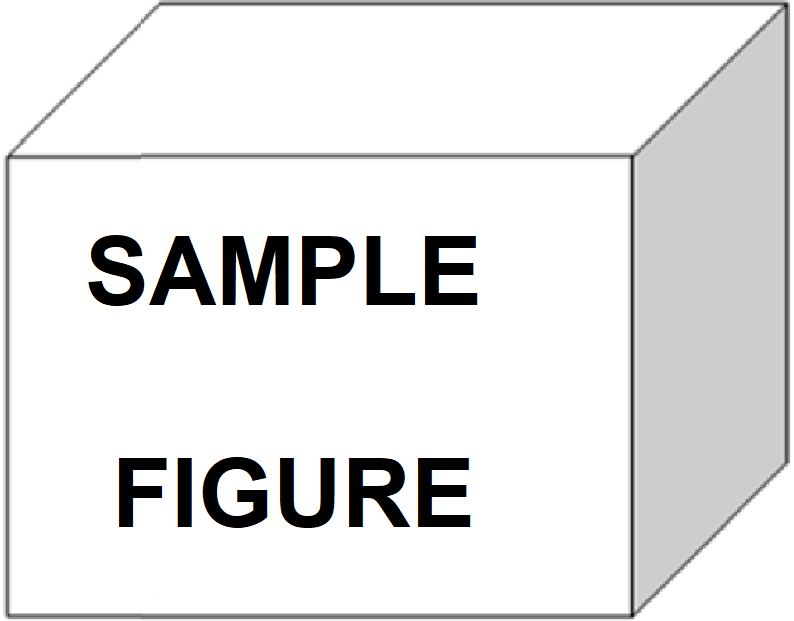
\includegraphics[width=10cm,keepaspectratio=true]{./fig/sekil1}
    % sekil1.eps: 0x0 pixel, 300dpi, 0.00x0.00 cm, bb=14 14 592 479
    \caption{Model structures.}
    \label{fig:ch1-1}
\end{figure}
\vspace{-6pt}

Lorem ipsum dolor sit amet, consectetur adipiscing elit. Praesent imperdiet, nisi 
nec aliquam cursus, dui turpis mollis nisl, ac consequat tellus sapien sit amet 
magna. Duis vel venenatis velit. Vestibulum ante ipsum primis in faucibus orci 
luctus et ultrices posuere cubilia Curae; Proin malesuada risus nec metus dapibus 
eu tincidunt lectus dignissim Figure \ref{fig:ch1-1}.

Lorem ipsum dolor sit amet, consectetur adipiscing elit. Praesent imperdiet, nisi 
nec aliquam cursus, dui turpis mollis nisl, ac consequat tellus sapien sit amet 
magna. Duis vel venenatis velit. Vestibulum ante ipsum primis in faucibus orci 
luctus et ultrices posuere cubilia Curae; Proin malesuada risus nec metus dapibus 
eu tincidunt lectus dignissim. 

\citet*{harper2007} lorem ipsum dolor sit amet, consectetur adipiscing elit. Table \ref{table:ch1-1} Praesent imperdiet, nisi 
nec aliquam cursus, dui turpis mollis nisl, ac consequat tellus sapien sit amet 
magna. Duis vel venenatis velit. Vestibulum ante ipsum primis in faucibus orci 
luctus et ultrices posuere cubilia Curae; Proin malesuada risus nec metus dapibus 
eu tincidunt lectus dignissim \cite{unesco}.

\vspace{3pt}
\begin{table}[ht]
\centering
\caption{Table captions must be ended with a full stop.}
\setlength{\tabcolsep}{14pt}
\begin{tabular}{cccc}
\toprule\midrule
Column A & Column B & Column C & Column D \\
\midrule
Row A & Row A & Row A & Row A \\
Row B & Row B & Row B & Row B \\
Row C & Row C & Row C & Row C \\
\bottomrule
\end{tabular}
\label{table:ch1-1}
\end{table}
\vspace{-6pt}

Lorem ipsum dolor sit amet, consectetur adipiscing elit. Praesent imperdiet, nisi 
nec aliquam cursus, dui turpis mollis nisl, ac consequat tellus sapien sit amet 
magna. Duis vel venenatis velit. Vestibulum ante ipsum primis in faucibus orci 
luctus et ultrices posuere cubilia Curae; Proin malesuada risus nec metus dapibus 
eu tincidunt lectus dignissim.Lorem ipsum dolor sit amet, consectetur adipiscing elit. 
Praesent imperdiet, nisi nec aliquam cursus, dui turpis mollis nisl, ac consequat 
tellus \cite{mccaffrey88, moore91, nelson88, sisaky, simpsondvd, startrek, TS-40561, url-1, url-2, vanden2001} 
%\cite{moore91} \cite{nelson88} \cite{sisaky} \cite{simpsondvd} \cite{startrek} \cite{TS-40561} \cite{url-1} \cite{url-2} \cite{vanden2001}.

Duis vel venenatis velit. Vestibulum ante ipsum primis in faucibus orci 
luctus et ultrices posuere cubilia Curae; Proin malesuada risus nec metus dapibus 
eu tincidunt lectus dignissim.

Lorem ipsum dolor sit amet, consectetur adipiscing elit. Praesent imperdiet, nisi 
nec aliquam cursus, dui turpis mollis nisl, ac consequat tellus sapien sit amet 
magna. Duis vel venenatis velit. Vestibulum ante ipsum primis in faucibus orci 
luctus et ultrices posuere cubilia Curae; Proin malesuada risus nec metus dapibus 
eu tincidunt lectus dignissim.

\citeauthor*{nelson88} (\citeyear{nelson88}) lorem ipsum dolor sit amet, consectetur adipiscing elit. Praesent imperdiet, nisi 
nec aliquam cursus, dui turpis mollis nisl, ac consequat tellus sapien sit amet 
magna. Duis vel venenatis velit. Vestibulum ante ipsum primis in faucibus orci 
luctus et ultrices posuere cubilia Curae; Proin malesuada risus nec metus dapibus 
eu tincidunt lectus dignissim .



%%%%%%%%%%%%%%%%%%%%%%%%%%%%%%%%%%%%%%%%%%%%%%%%%%%%%%%%%%%%%%%%%
\chapter{TABLES AND FIGURES}\label{CH2}
%%%%%%%%%%%%%%%%%%%%%%%%%%%%%%%%%%%%%%%%%%%%%%%%%%%%%%%%%%%%%%%%%

\vspace{6pt}

\section{Figure Citations and Figure Example}

Tables and figures given in appendices must be numbered with the number of the appendix they are in (i.e. \textbf{Table A.1}, \textbf{Table A.2}, \textbf{Figure A.1}, \textbf{Figure A.2}).

In tables and figures, font size could be reduced to 8 pt, if necessary.

Tables must be prepared using the same font type as the thesis. The font type used in figures must be consistent throughout the thesis.

Tables and figures must be placed after they are first cited in the main text body, but must be as close as possible, in accordance with the rules in this guideline such as \figurename\ \ref{fig:ch2-1}. All tables and figures must be cited before they are used in the main text body.

All tables and figures must be horizontally centered on the page.

\vspace{6pt} % 12pt
\begin{figure}[!ht]
    \centering
    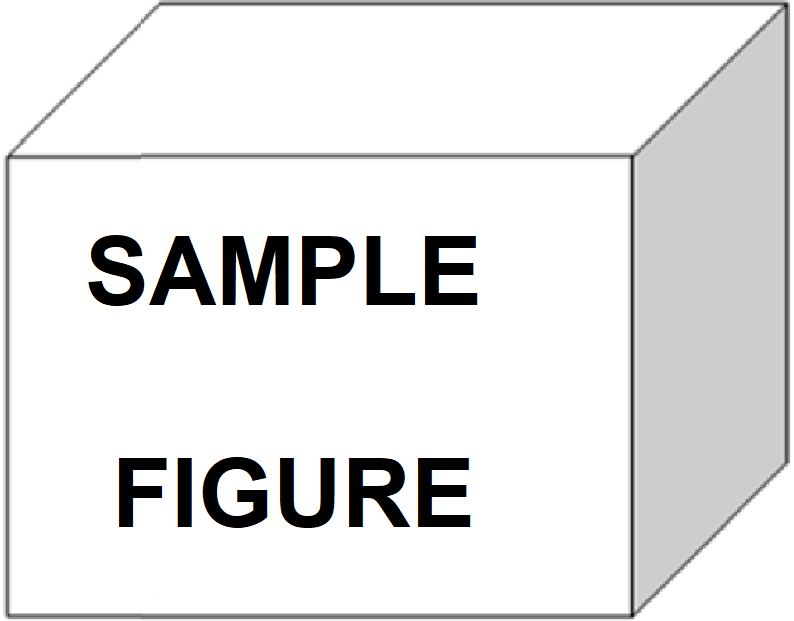
\includegraphics[width=5cm,keepaspectratio=true]{./fig/sekil1.png}
    % sekil2.eps: 0x0 pixel, 300dpi, 0.00x0.00 cm, bb=14 14 818 556
    \caption{All tables and figures must be horizontally centered on the page.}
    \label{fig:ch2-1}
\end{figure}
\vspace{-6pt}

The numbering of the tables and the figures must be such that the first number is the number of the chapter the table/figure is placed under (for appendices, the letter of the appendix), and the second number is the number of order (i.e. Table 1.2, Figure 3.5, Table A.1, Figure B.5). The words “Table” and “Figure” and numbers must be bold.

For table numbers and captions, 1 line spacing, 12 pt (before) and 6 pt (after) paragraph spacing must be set. Table captions must be ended with a full stop. A table and its caption must be on the same page. \vfill\phantom{.}

Multiple tables/figures could be placed on one page, however, table/figures spanning more than 4 consecutive pages must be given in appendices rather than the main text body.

The first paragraph following a table must have 12 pt (before) and 6 pt (after) paragraph spacing. Titles following a table must have the standard formatting as previously specified. 

Footnotes for a table must be written with 1 line spacing and a font size 2 pt smaller than the main text body. 

For figure numbers and captions, 1 line spacing, 6 pt (before) and 12 pt (after) paragraph spacing must be set. Figure captions must be ended with a full stop. A figure and its caption must be on the same page. 

For figures spanning more than one page, the same number and caption must be written below the continued figure, with the expression ”continued” added in brackets (i.e. \textbf{Table 1.1 (continued):} Metal composition of wastes. \textbf{Figure 1.1 (continued):} Water supply network of ISTANBUL.).

Plots, images and musical notes must be numbered and captioned as figures. Musical notes must be written according to the format rules set by the İTU School of Traditional Turkish Music. 

It is recommended that elements that increase the page thickness and disrupt the binding structure of theses such as  folded pages or additional items embedded on pages are given as appendices.

\figurename\ \ref{fig:ch2-2} Sed diam nonumy eirmod tempor invidunt ut labore et dolore magna aliquyam erat, sed diam voluptua. At vero eos et accusam et justo duo dolores et ea rebum. Lorem ipsum dolor sit amet, consetetur sadipscing elitr, sed diam nonumy eirmod tempor invidunt ut labore et dolore magna aliquyam erat, sed diam voluptua. At vero eos et accusam et justo duo dolores et ea rebum. At vero eos et accusam et justo duo dolores et ea rebum. At vero eos et accusam et justo duo dolores et ea rebum. At vero eos et accusam et justo duo dolores et ea rebum. At vero eos et accusam et justo duo dolores et ea rebum. At vero eos et accusam et justo duo dolores et ea rebum. At vero eos et accusam et justo duo dolores et ea rebum. \vfill\phantom{.}

Lorem ipsum dolor sit amet, consetetur sadipscing elitr, sed diam nonumy eirmod tempor invidunt ut labore et dolore magna aliquyam erat, sed diam voluptua. At vero eos et accusam et justo duo dolores et ea rebum. At vero eos et accusam et justo duo dolores et ea rebum. At vero eos et accusam et justo duo dolores et ea rebum.

\vspace{6pt} % 12pt
\begin{figure}[ht]
    \centering
    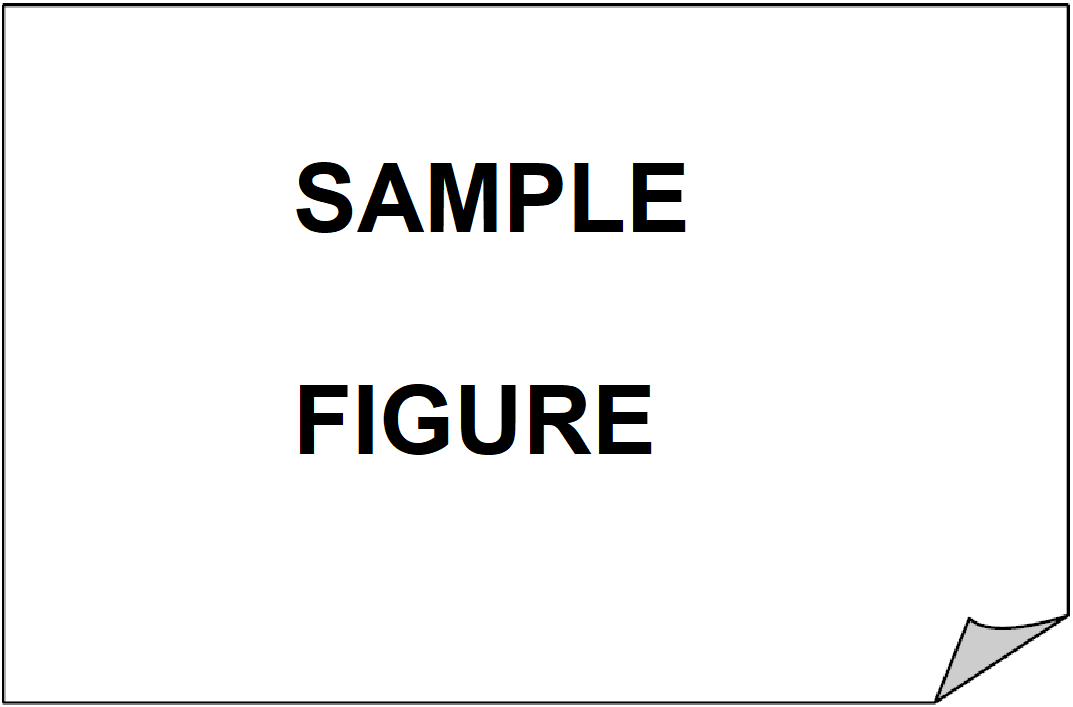
\includegraphics[width=10cm,keepaspectratio=true]{./fig/sekil2.png}
    % sekil2.eps: 0x0 pixel, 300dpi, 0.00x0.00 cm, bb=14 14 818 556
    \caption{Example figure.}
    \label{fig:ch2-2}
\end{figure}
\vspace{-6pt} % 12pt

\section{Landscape-oriented, full-page figure}

Lorem ipsum dolor sit amet, consetetur sadipscing elitr, sed diam nonumy eirmod tempor invidunt ut labore et dolore magna aliquyam erat, sed diam voluptua. At vero eos et accusam et justo duo dolores et ea rebum (\figurename\ \ref{fig:ch2-3}). Lorem ipsum dolor sit amet, consetetur sadipscing elitr, sed diam nonumy eirmod tempor invidunt ut labore et dolore magna aliquyam erat, sed diam voluptua. At vero eos et accusam et justo duo dolores et ea rebum. 

Lorem ipsum dolor sit amet, consetetur sadipscing elitr, sed diam nonumy eirmod tempor invidunt ut labore et dolore magna aliquyam erat, sed diam voluptua. At vero eos et accusam et justo duo dolores et ea rebum. Lorem ipsum dolor sit amet, consetetur sadipscing elitr, sed diam nonumy eirmod tempor invidunt ut labore et dolore magna aliquyam erat, sed diam voluptua. At vero eos et accusam et justo duo dolores et ea rebum. Lorem ipsum dolor sit amet, consetetur sadipscing elitr, sed diam nonumy eirmod tempor invidunt ut labore et dolore magna aliquyam erat, sed diam voluptua. At vero eos et accusam et justo duo dolores et ea rebum.   

\begin{landscape}
\thispagestyle{empty}
\vspace{6pt}
\begin{figure}[htp!]
      \centering
      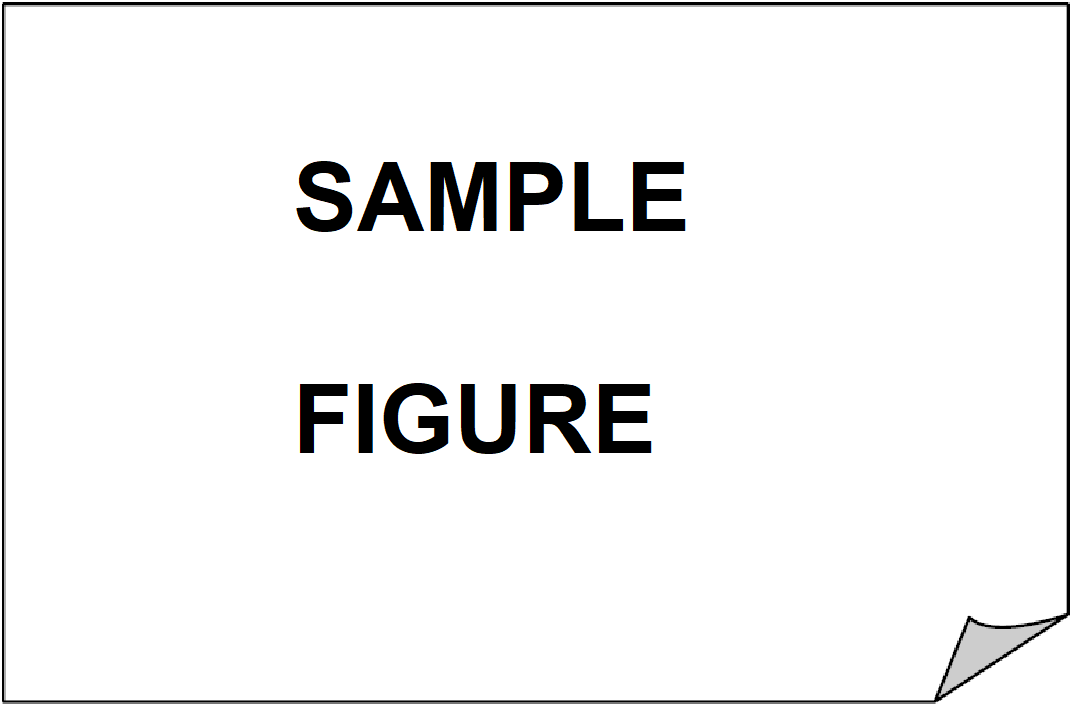
\includegraphics[width=500pt,keepaspectratio=true]{./fig/sekil3.png}
      % sekil3.eps: 0x0 pixel, 300dpi, 0.00x0.00 cm, bb=14 14 1155 740
      \caption{Landscape-oriented, full-page figure.}    
      \label{fig:ch2-3}
\end{figure}
\vspace{-6pt}
\vfill\hbox{ }

\ifodd\value{page} % Tek sf
\begin{textblock*}{1cm}[0,0](19.5cm,14.85cm) % 210 - 15
\else		% Cift sf
\begin{textblock*}{1cm}[0,0](18.0cm,14.85cm) % 210 - 30
\fi
{\rotatebox{90}{\centering\thepage}} % sf numarası
\end{textblock*}
\end{landscape}

Lorem ipsum dolor sit amet, consetetur sadipscing elitr, sed diam nonumy eirmod tempor invidunt ut labore et dolore magna aliquyam erat, sed diam voluptua. At vero eos et accusam et justo duo dolores et ea rebum. Lorem ipsum dolor sit amet, consetetur sadipscing elitr, sed diam nonumy eirmod tempor invidunt ut labore et dolore magna aliquyam erat, sed diam voluptua. At vero eos et accusam et justo duo dolores et ea rebum. Lorem ipsum dolor sit amet, consetetur sadipscing elitr, sed diam nonumy eirmod tempor invidunt ut labore et dolore magna aliquyam erat, sed diam voluptua. At vero eos et accusam et justo duo dolores et ea rebum. Lorem ipsum dolor sit amet, consetetur sadipscing elitr, sed diam nonumy eirmod tempor invidunt ut labore et dolore magna aliquyam erat, sed diam voluptua. At vero eos et accusam et justo duo dolores et ea rebum.

\section{Table Citations and Table Example}

Lorem ipsum dolor sit amet, consetetur sadipscing elitr, sed diam nonumy eirmod tempor invidunt ut labore et dolore magna aliquyam erat, sed diam voluptua. At vero eos et accusam et justo duo dolores et ea rebum. Stet clita kasd gub rgren, no sea takimata sanctus est Lorem ipsum dolor sit amet, consetetur sadipscing elitr, sed diam nonumy eirmod tempor invidunt ut lab ore sit et dolore magna.

As seen in \tablename\ \ref{table:ch2-1} lorem ipsum dolor sit amet, consetetur sadipscing elitr, sed diam nonumy eirmod tempor invidunt ut labore et dolore magna aliquyam erat, sed diam voluptua. At vero eos et accusam et justo duo dolores et ea rebum. Stet clita kasd gub rgren, no sea takimata sanctus est Lorem ipsum dolor sit amet, consetetur sadipscing elitr, sed diam nonumy eirmod tempor invidunt ut lab ore sit et dolore magna.

\vspace{6pt} 
\begin{table}[!ht]
\centering
\setlength{\tabcolsep}{14pt}
\caption{Table captions must be ended with a full stop.}
\begin{tabular}{cccc}
\toprule\midrule
Column A & Column B & Column C & Column D \\
\midrule
Row A & Row A & Row A & Row A \\
Row B & Row B & Row B & Row B \\
Row C & Row C & Row C & Row C \\
\bottomrule
\end{tabular}
\label{table:ch2-1}
\end{table}
\vspace{-6pt} 

Lorem ipsum dolor sit amet, consetetur sadipscing elitr, sed diam nonumy eirmod tempor invidunt ut labore et dolore magna aliquyam erat, sed diam voluptua. At vero eos et accusam et justo duo dolores et ea rebum. 

Lorem ipsum dolor sit amet, consetetur sadipscing elitr, sed diam nonumy eirmod tempor invidunt ut labore et dolore magna aliquyam erat, sed diam voluptua. At vero eos et accusam et justo duo dolores et ea rebum. Stet clita kasd gub rgren, no sea takimata sanctus est Lorem ipsum dolor sit amet, consetetur sadipscing elitr, sed diam nonumy eirmod tempor invidunt ut lab ore sit et dolore magna. Lorem ipsum dolor sit amet, consetetur sadipscing elitr, sed diam nonumy eirmod tempor invidunt ut labore et dolore magna aliquyam erat, sed diam voluptua. At vero eos et accusam et justo duo dolores et ea rebum \tablename\ \ref{table:ch2-2}.

\vspace{6pt} % 12pt
\begin{table}[!ht]
\centering
\setlength{\tabcolsep}{14pt}
\caption{Table captions must be ended with a full stop.}
\begin{tabular}{cccc}
\toprule\midrule
Column A & Column B & Column C & Column D \\
\midrule
Row A & Row A & Row A & Row A \\
Row B & Row B & Row B & Row B \\
Row C & Row C & Row C & Row C \\
\bottomrule
\end{tabular}
\label{table:ch2-2}
\end{table}
\vspace{-6pt} % 12pt 

Lorem ipsum dolor sit amet, consetetur sadipscing elitr, sed diam nonumy eirmod tempor invidunt ut labore et dolore magna aliquyam erat, sed diam voluptua. At vero eos et accusam et justo duo dolores et ea rebum. Stet clita kasd gub rgren, no sea takimata sanctus est Lorem ipsum dolor sit amet, consetetur sadipscing elitr, sed diam nonumy eirmod tempor invidunt ut lab ore sit et dolore magna. Lorem ipsum dolor sit amet, consetetur sadipscing elitr, sed diam nonumy eirmod tempor invidunt ut labore et dolore magna aliquyam erat, sed diam voluptua. At vero eos et accusam et justo duo dolores et ea rebum. 

\section{Landscape-oriented, full-page table}

Lorem ipsum dolor sit amet, consetetur sadipscing elitr, sed diam nonumy eirmod tempor invidunt ut labore et dolore magna aliquyam erat, sed diam voluptua. At vero eos et accusam et justo duo dolores et ea rebum. Stet clita kasd gub rgren, no sea takimata sanctus est Lorem ipsum dolor sit amet, consetetur sadipscing elitr, sed diam nonumy eirmod tempor invidunt ut lab ore sit et dolore magna \tablename\ \ref{table:ch2-3}. \vfill\phantom{.}

\begin{landscape}
\thispagestyle{empty}
\vspace{6pt} % 12pt
\begin{table}[htp]
\centering
\setlength{\tabcolsep}{14pt}
\captionsetup{justification=centerlast}
\caption{Captioning in landscape-oriented pages: the most important aspect is to align the lines horizontally.}
\label{table:ch2-3}
\begin{tabular}{lccrrrrr}
\toprule\midrule
\multirow{2}{*}{Parametre} & \multirow{2}{*}{Column 2} & \multirow{2}{*}{Column 3} & \multicolumn{3}{c}{Column 4} & \multicolumn{2}{c}{Column 5}\\ \cmidrule(lr){4-6} \cmidrule(lr){7-8}
  & & & Subcolumn & Subcolumn & Subcolumn & Subcolumn & Subcolumn\\
\midrule
Row 1 & -7.680442 & 7.6986348 & 0.00 & 0.00 & 0.00 & 12 & 12 \\
Row 2 & 140 & - & 0.50 & 0.00 & 0.00 & 0 & 0 \\
Row 3 & 37.174357 & 37.16192697 & 0.00 & 0.00 & 0.00 & 0 & 24 \\
Row 4 & 140 & - & 0.50 & 0.00 & 0.00 & 0 & 0 \\
Row 5 & 37.174357 & 37.16192697 & 0.00 & 0.00 & 0.00 & 0 & 24 \\
Row 6 & 140 & - & 0.50 & 0.00 & 0.00 & 0 & 0 \\
Row 7 & 37.174357 & 37.16192697 & 0.00 & 0.00 & 0.00 & 0 & 24 \\
Row 8 & 140 & - & 0.50 & 0.00 & 0.00 & 0 & 0 \\
Row 9 & 37.174357 & 37.16192697 & 0.00 & 0.00 & 0.00 & 0 & 24 \\
Row 10 & 140 & - & 0.50 & 0.00 & 0.00 & 0 & 0 \\
Row 11 & 37.174357 & 37.16192697 & 0.00 & 0.00 & 0.00 & 0 & 24 \\
Row 12 & 140 & - & 0.50 & 0.00 & 0.00 & 0 & 0 \\
Row 13 & 37.174357 & 37.16192697 & 0.00 & 0.00 & 0.00 & 0 & 24 \\
Row 14 & 140 & - & 0.50 & 0.00 & 0.00 & 0 & 0 \\
Row 15 & 37.174357 & 37.16192697 & 0.00 & 0.00 & 0.00 & 0 & 24 \\
\bottomrule
\end{tabular}
\end{table}
\vspace{-6pt} % 12pt 
\vfill\hbox{ }

\ifodd\value{page} % Tek sf
\begin{textblock*}{1cm}[0,0](19.5cm,14.85cm) % 210 - 15
\else		% Cift sf
\begin{textblock*}{1cm}[0,0](18.0cm,14.85cm) % 210 - 30
\fi
{\rotatebox{90}{\centering\thepage}} % sf numarası
\end{textblock*}
\end{landscape}

\begin{landscape}
\thispagestyle{empty}
\vspace{6pt} % 12pt
\begin{table}[htp]
\centering
\setlength{\tabcolsep}{14pt}
\captionsetup{justification=centerlast}
\caption*{\textbf{\tablename\ \ref{table:ch2-3} (continued) : } Captioning in landscape-oriented pages: the most important aspect is to align the lines horizontally.}
\begin{tabular}{lccrrrrr}
\toprule\midrule
\multirow{2}{*}{Parametre} & \multirow{2}{*}{Column 2} & \multirow{2}{*}{Column 3} & \multicolumn{3}{c}{Column 4} & \multicolumn{2}{c}{Column 5}\\ \cmidrule(lr){4-6} \cmidrule(lr){7-8}
  & & & Subcolumn & Subcolumn & Subcolumn & Subcolumn & Subcolumn\\
\midrule
Row 1 & -7.680442 & 7.6986348 & 0.00 & 0.00 & 0.00 & 12 & 12 \\
Row 2 & 140 & - & 0.50 & 0.00 & 0.00 & 0 & 0 \\
Row 3 & 37.174357 & 37.16192697 & 0.00 & 0.00 & 0.00 & 0 & 24 \\
Row 4 & 140 & - & 0.50 & 0.00 & 0.00 & 0 & 0 \\
Row 5 & 37.174357 & 37.16192697 & 0.00 & 0.00 & 0.00 & 0 & 24 \\
Row 6 & 140 & - & 0.50 & 0.00 & 0.00 & 0 & 0 \\
Row 7 & 37.174357 & 37.16192697 & 0.00 & 0.00 & 0.00 & 0 & 24 \\
Row 8 & 140 & - & 0.50 & 0.00 & 0.00 & 0 & 0 \\
Row 9 & 37.174357 & 37.16192697 & 0.00 & 0.00 & 0.00 & 0 & 24 \\
Row 10 & 140 & - & 0.50 & 0.00 & 0.00 & 0 & 0 \\
Row 11 & 37.174357 & 37.16192697 & 0.00 & 0.00 & 0.00 & 0 & 24 \\
Row 12 & 140 & - & 0.50 & 0.00 & 0.00 & 0 & 0 \\
Row 13 & 37.174357 & 37.16192697 & 0.00 & 0.00 & 0.00 & 0 & 24 \\
Row 14 & 140 & - & 0.50 & 0.00 & 0.00 & 0 & 0 \\
Row 15 & 37.174357 & 37.16192697 & 0.00 & 0.00 & 0.00 & 0 & 24 \\
\bottomrule
\end{tabular}
\end{table}
\vspace{-6pt} % 12pt 
\vfill\hbox{ }

\ifodd\value{page} % Tek sf
\begin{textblock*}{1cm}[0,0](19.5cm,14.85cm) % 210 - 15
\else		% Cift sf
\begin{textblock*}{1cm}[0,0](18.0cm,14.85cm) % 210 - 30
\fi
{\rotatebox{90}{\centering\thepage}} % sf numarası
\end{textblock*}
\end{landscape}

\section{Alternative full-page long table}

Lorem ipsum dolor sit amet, consetetur sadipscing elitr, sed diam nonumy eirmod tempor invidunt ut labore et dolore magna aliquyam erat, sed diam voluptua. At vero eos et accusam et justo duo dolores et ea rebum. Lorem ipsum dolor sit amet, consetetur sadipscing elitr, sed diam nonumy eirmod tempor invidunt ut labore et dolore magna aliquyam erat, sed diam voluptua. At vero eos et accusam et justo duo dolores et ea rebum. Lorem ipsum dolor sit amet, consetetur sadipscing elitr, sed diam nonumy eirmod tempor invidunt ut labore et dolore magna aliquyam erat, sed diam voluptua. At vero eos et accusam et justo duo dolores et ea rebum \tablename\ \ref{table:ch2-4}.

\vspace{6pt} % 12pt
\begin{small}
\begin{longtable}{ccc}
		%Here is the caption, the stuff in [] is the table of contents entry,
		%the stuff in {} is the title that will appear on the first page of the
		%table.
		\caption{An example of a longtable table which is a long table.}\label{table:ch2-4}\\
		%This is the header for the first page of the table...
		\toprule\midrule
		\multicolumn{1}{c}{{Time (s)}} &
		\multicolumn{1}{c}{{Triple chosen}} &
		\multicolumn{1}{c}{{Other feasible triples}} \\
		\midrule
		\endfirsthead
		
		%This is the header for the remaining page(s) of the table...
		\caption*{\textbf{\tablename\ \thetable\ (continued) :} An example of a longtable table which is a long table.} \\ 
		\toprule \midrule
		\multicolumn{1}{c}{{Time (s)}} &
		\multicolumn{1}{c}{{Triple chosen}} &
		\multicolumn{1}{c}{{Other feasible triples}} \\
		\midrule
		\endhead
		
		%This is the footer for all pages except the last page of the table...
		%\multicolumn{3}{l}{{Continued on Next Page\ldots}} \\
		\bottomrule
		\endfoot
		
		%This is the footer for the last page of the table...
		\bottomrule
		\endlastfoot
		
		%Now the data...
		0      & (1, 11, 13725) & (1, 12, 10980), (1, 13, 8235), (2, 2, 0), (3, 1, 0) \\
		2745   & (1, 12, 10980) & (1, 13, 8235), (2, 2, 0), (2, 3, 0), (3, 1, 0) \\
		5490   & (1, 12, 13725) & (2, 2, 2745), (2, 3, 0), (3, 1, 0) \\
		8235   & (1, 12, 16470) & (1, 13, 13725), (2, 2, 2745), (2, 3, 0), (3, 1, 0) \\
		% <data removed>
		164700 & (1, 13, 13725) & (2, 2, 2745), (2, 3, 0), (3, 1, 0) \\
		0      & (1, 11, 13725) & (1, 12, 10980), (1, 13, 8235), (2, 2, 0), (3, 1, 0) \\
		2745   & (1, 12, 10980) & (1, 13, 8235), (2, 2, 0), (2, 3, 0), (3, 1, 0) \\
		5490   & (1, 12, 13725) & (2, 2, 2745), (2, 3, 0), (3, 1, 0) \\
		8235   & (1, 12, 16470) & (1, 13, 13725), (2, 2, 2745), (2, 3, 0), (3, 1, 0) \\
		% <data removed>
		164700 & (1, 13, 13725) & (2, 2, 2745), (2, 3, 0), (3, 1, 0) \\
		0      & (1, 11, 13725) & (1, 12, 10980), (1, 13, 8235), (2, 2, 0), (3, 1, 0) \\
		2745   & (1, 12, 10980) & (1, 13, 8235), (2, 2, 0), (2, 3, 0), (3, 1, 0) \\
		5490   & (1, 12, 13725) & (2, 2, 2745), (2, 3, 0), (3, 1, 0) \\
		8235   & (1, 12, 16470) & (1, 13, 13725), (2, 2, 2745), (2, 3, 0), (3, 1, 0) \\
		% <data removed>
		164700 & (1, 13, 13725) & (2, 2, 2745), (2, 3, 0), (3, 1, 0) \\
		0      & (1, 11, 13725) & (1, 12, 10980), (1, 13, 8235), (2, 2, 0), (3, 1, 0) \\
		2745   & (1, 12, 10980) & (1, 13, 8235), (2, 2, 0), (2, 3, 0), (3, 1, 0) \\
		5490   & (1, 12, 13725) & (2, 2, 2745), (2, 3, 0), (3, 1, 0) \\
		8235   & (1, 12, 16470) & (1, 13, 13725), (2, 2, 2745), (2, 3, 0), (3, 1, 0) \\
		% <data removed>
		164700 & (1, 13, 13725) & (2, 2, 2745), (2, 3, 0), (3, 1, 0) \\
		0      & (1, 11, 13725) & (1, 12, 10980), (1, 13, 8235), (2, 2, 0), (3, 1, 0) \\
		2745   & (1, 12, 10980) & (1, 13, 8235), (2, 2, 0), (2, 3, 0), (3, 1, 0) \\
		5490   & (1, 12, 13725) & (2, 2, 2745), (2, 3, 0), (3, 1, 0) \\
		8235   & (1, 12, 16470) & (1, 13, 13725), (2, 2, 2745), (2, 3, 0), (3, 1, 0) \\
		% <data removed>
		164700 & (1, 13, 13725) & (2, 2, 2745), (2, 3, 0), (3, 1, 0) \\
		0      & (1, 11, 13725) & (1, 12, 10980), (1, 13, 8235), (2, 2, 0), (3, 1, 0) \\
		2745   & (1, 12, 10980) & (1, 13, 8235), (2, 2, 0), (2, 3, 0), (3, 1, 0) \\
		5490   & (1, 12, 13725) & (2, 2, 2745), (2, 3, 0), (3, 1, 0) \\
		8235   & (1, 12, 16470) & (1, 13, 13725), (2, 2, 2745), (2, 3, 0), (3, 1, 0) \\
		% <data removed>
		164700 & (1, 13, 13725) & (2, 2, 2745), (2, 3, 0), (3, 1, 0) \\
		0      & (1, 11, 13725) & (1, 12, 10980), (1, 13, 8235), (2, 2, 0), (3, 1, 0) \\
		2745   & (1, 12, 10980) & (1, 13, 8235), (2, 2, 0), (2, 3, 0), (3, 1, 0) \\
		5490   & (1, 12, 13725) & (2, 2, 2745), (2, 3, 0), (3, 1, 0) \\
		8235   & (1, 12, 16470) & (1, 13, 13725), (2, 2, 2745), (2, 3, 0), (3, 1, 0) \\
		% <data removed>
		164700 & (1, 13, 13725) & (2, 2, 2745), (2, 3, 0), (3, 1, 0) \\
		0      & (1, 11, 13725) & (1, 12, 10980), (1, 13, 8235), (2, 2, 0), (3, 1, 0) \\
		2745   & (1, 12, 10980) & (1, 13, 8235), (2, 2, 0), (2, 3, 0), (3, 1, 0) \\
		5490   & (1, 12, 13725) & (2, 2, 2745), (2, 3, 0), (3, 1, 0) \\
		8235   & (1, 12, 16470) & (1, 13, 13725), (2, 2, 2745), (2, 3, 0), (3, 1, 0) \\
		% <data removed>
		164700 & (1, 13, 13725) & (2, 2, 2745), (2, 3, 0), (3, 1, 0) \\
		0      & (1, 11, 13725) & (1, 12, 10980), (1, 13, 8235), (2, 2, 0), (3, 1, 0) \\
		2745   & (1, 12, 10980) & (1, 13, 8235), (2, 2, 0), (2, 3, 0), (3, 1, 0) \\
		5490   & (1, 12, 13725) & (2, 2, 2745), (2, 3, 0), (3, 1, 0) \\
		8235   & (1, 12, 16470) & (1, 13, 13725), (2, 2, 2745), (2, 3, 0), (3, 1, 0) \\
		% <data removed>
		164700 & (1, 13, 13725) & (2, 2, 2745), (2, 3, 0), (3, 1, 0) \\
		0      & (1, 11, 13725) & (1, 12, 10980), (1, 13, 8235), (2, 2, 0), (3, 1, 0) \\
		2745   & (1, 12, 10980) & (1, 13, 8235), (2, 2, 0), (2, 3, 0), (3, 1, 0) \\
		5490   & (1, 12, 13725) & (2, 2, 2745), (2, 3, 0), (3, 1, 0) \\
		8235   & (1, 12, 16470) & (1, 13, 13725), (2, 2, 2745), (2, 3, 0), (3, 1, 0) \\
		% <data removed>
		164700 & (1, 13, 13725) & (2, 2, 2745), (2, 3, 0), (3, 1, 0) \\
		0      & (1, 11, 13725) & (1, 12, 10980), (1, 13, 8235), (2, 2, 0), (3, 1, 0) \\
		2745   & (1, 12, 10980) & (1, 13, 8235), (2, 2, 0), (2, 3, 0), (3, 1, 0) \\
		5490   & (1, 12, 13725) & (2, 2, 2745), (2, 3, 0), (3, 1, 0) \\
		8235   & (1, 12, 16470) & (1, 13, 13725), (2, 2, 2745), (2, 3, 0), (3, 1, 0) \\
		% <data removed>
		164700 & (1, 13, 13725) & (2, 2, 2745), (2, 3, 0), (3, 1, 0) \\
		0      & (1, 11, 13725) & (1, 12, 10980), (1, 13, 8235), (2, 2, 0), (3, 1, 0) \\
		2745   & (1, 12, 10980) & (1, 13, 8235), (2, 2, 0), (2, 3, 0), (3, 1, 0) \\
		5490   & (1, 12, 13725) & (2, 2, 2745), (2, 3, 0), (3, 1, 0) \\
		8235   & (1, 12, 16470) & (1, 13, 13725), (2, 2, 2745), (2, 3, 0), (3, 1, 0) \\
		% <data removed>
		164700 & (1, 13, 13725) & (2, 2, 2745), (2, 3, 0), (3, 1, 0) \\
		0      & (1, 11, 13725) & (1, 12, 10980), (1, 13, 8235), (2, 2, 0), (3, 1, 0) \\
		2745   & (1, 12, 10980) & (1, 13, 8235), (2, 2, 0), (2, 3, 0), (3, 1, 0) \\
		5490   & (1, 12, 13725) & (2, 2, 2745), (2, 3, 0), (3, 1, 0) \\
		8235   & (1, 12, 16470) & (1, 13, 13725), (2, 2, 2745), (2, 3, 0), (3, 1, 0) \\
\end{longtable}
\end{small}
\vspace{-6pt} % 12pt 

Lorem ipsum dolor sit amet, consetetur sadipscing elitr, sed diam nonumy eirmod tempor invidunt ut labore et dolore magna aliquyam erat, sed diam voluptua. At vero eos et accusam et justo duo dolores et ea rebum. Lorem ipsum dolor sit amet, consetetur sadipscing elitr, sed diam nonumy eirmod tempor invidunt ut labore et dolore magna aliquyam erat, sed diam voluptua. At vero eos et accusam et justo duo dolores et ea rebum. Lorem ipsum dolor sit amet, consetetur sadipscing elitr, sed diam nonumy eirmod tempor invidunt ut labore et dolore magna aliquyam erat, sed diam voluptua. At vero eos et accusam et justo duo dolores et ea rebum. 
%%%%%%%%%%%%%%%%%%%%%%%%%%%%%%%%%%%%%%%%%%%%%%%%%%%%%%%%%%%%%%%%%
\chapter{MAIN TEXT BODY}\label{ch:ch3}
%%%%%%%%%%%%%%%%%%%%%%%%%%%%%%%%%%%%%%%%%%%%%%%%%%%%%%%%%%%%%%%%%

\vspace{-12pt} %iki başlık alt alta. iki katı boşluk olmasın

\section{Body Texts}

Lorem ipsum dolor sit amet, consetetur sadipscing elitr, sed diam nonumy eirmod tempor invidunt ut labore et dolore magna aliquyam erat, sed diam voluptua. At vero eos et accusam et justo duo dolores et ea rebum. Stet clita kasd gub rgren, no sea takimata sanctus est Lorem ipsum dolor sit amet, consetetur sadipscing elitr, sed diam nonumy eirmod tempor invidunt ut lab ore sit et dolore magna.

Lorem ipsum dolor sit amet, consetetur sadipscing elitr, sed diam nonumy eirmod tempor invidunt ut labore et dolore magna aliquyam erat, sed diam voluptua. At vero eos et accusam et justo duo dolores et ea rebum. Stet clita kasd gub rgren, no sea takimata sanctus est Lorem ipsum dolor sit amet, consetetur sadipscing elitr, sed diam nonumy eirmod tempor invidunt ut lab ore sit et dolore magna.

\subsection{Page Margins}

Lorem ipsum dolor sit amet, consetetur sadipscing elitr, sed diam Lorem ipsum dolor sit amet, consetetur sadipscing elitr, sed diam nonumy eirmod tempor invidunt ut labore et dolore magna aliquyam erat, sed diam voluptua. At vero eos et accusam et justo duo dolores et ea rebum (\figurename\ \ref{fig:ch3-1}.).

\vspace{6pt} % 12pt
\begin{figure}[!ht]
      \centering
      
\includegraphics[width=230pt,keepaspectratio=true]{./fig/sekil3}
      % sekil3.eps: 0x0 pixel, 300dpi, 0.00x0.00 cm, bb=14 14 1155 740
      \caption[Short version for LoF]{Long version to appear next to the figure.}
      \label{fig:ch3-1}
\end{figure}
\vspace{-9pt} % 12pt 

Lorem ipsum dolor sit amet, consetetur sadipscing elitr, sed diam nonumy eirmod tempor invidunt ut labore et dolore magna aliquyam erat, sed diam voluptua. At vero eos et accusam et justo duo dolores et ea rebum. Stet clita kasd gub rgren, no sea takimata sanctus est Lorem ipsum dolor sit amet, consetetur sadipscing elitr, sed diam nonumy eirmod tempor invidunt ut lab ore sit et dolore magna.
At vero eos et accusam et justo duo dolores et ea rebum. Stet clita kasd gub rgren, no sea takimata sanctus est Lorem ipsum dolor sit amet, consetetur sadipscing elitr, sed diam nonumy eirmod tempor invidunt ut lab ore sit et dolore magna.
Lorem ipsum dolor sit amet, consetetur sadipscing elitr, sed diam nonumy eirmod tempor invidunt ut labore et dolore magna aliquyam erat, sed diam voluptua. At vero eos et accusam et justo duo dolores et ea rebum. Stet clita kasd gub rgren, no sea takimata sanctus est Lorem ipsum dolor sit amet, consetetur sadipscing elitr, sed diam nonumy eirmod tempor invidunt ut lab ore sit et dolore magna.

\subsection{Equations}

Lorem ipsum dolor sit amet, consetetur sadipscing elitr, sed diam nonumy eirmod tempor invidunt ut labore et dolore magna aliquyam erat, sed diam voluptua. At vero eos et accusam et justo duo dolores et ea rebum. Stet clita kasd gub rgren, no sea takimata sanctus est  Lorem ipsum dolor sit amet, consetetur sadipscing elitr,  sed diam nonumy eirmod tempor invidunt ut lab  ore sit et dolore magna Equation \eqref{eq:ch3-1}.
% 6pt boşluk için satır atlanmaması lazım
\begin{equation}
\label{eq:ch3-1}
   y_{t}  \equiv \phi_{1} y_{t-1} + \epsilon_{t}
\end{equation}
%
Each parameter is described. As seen in Equation \eqref{eq:ch3-1}, or in \eqref{eq:ch3-1}. Lorem ipsum dolor sit amet, consetetur sadipscing elitr, sed diam nonumy eirmod tempor invidunt ut labore et dolore magna aliquyam erat.

\subsection{Process based model: SWAT}

Lorem ipsum dolor sit amet, consetetur sadipscing elitr, sed diam nonumy eirmod tempor invidunt ut labore et dolore magna aliquyam erat, sed diam voluptua. At vero eos et accusam et justo duo dolores et ea rebum. Stet clita kasd gub rgren, no sea takimata sanctus est Lorem ipsum dolor sit amet, consetetur sadipscing elitr, sed diam nonumy eirmod tempor invidunt ut lab ore sit et dolore magna.

\figurename\ \ref{fig:ch3-2} Sed et est vestibulum felis sagittis congue. Phasellus fringilla sem eu purus posuere ut viverra massa dignissim. Maecenas ornare neque velit. Vivamus interdum  euismod elementum. Ut sit amet luctus ligula. Vivamus porttitor venenatis sem nec  congue. Quisque sed lectus et nibh imperdiet vestibulum. Vivamus vel turpis leo.  Proin suscipit iaculis nibh, nec dictum augue aliquet in. Praesent fermentum sem  tempus orci molestie at facilisis dui sagittis. Etiam sit amet imperdiet sapien.

\vspace{6pt} % 12pt
\begin{figure}[!ht]
      \centering
      
\includegraphics[width=230pt,keepaspectratio=true]{./fig/sekil3}
      % sekil3.eps: 0x0 pixel, 300dpi, 0.00x0.00 cm, bb=14 14 1155 740
      \vspace{4mm}
      \caption{For a multi-line figure captions, it is important that all the
      lines of the caption are aligned.}
      \label{fig:ch3-2}
\end{figure}
\vspace{-9pt} % 12pt 

Lorem ipsum dolor sit amet, consetetur sadipscing elitr, sed diam nonumy eirmod tempor invidunt ut labore et dolore magna aliquyam erat, sed diam voluptua. At vero eos et accusam et justo duo dolores et ea rebum. Stet clita kasd gub rgren, no sea takimata sanctus est Lorem ipsum dolor sit amet, consetetur sadipscing elitr, sed diam nonumy eirmod tempor invidunt ut lab ore sit et dolore magna.

tempor invidunt ut labore et dolore magna aliquyam erat, sed diam voluptua. At vero eos et accusam et justo duo dolores et ea rebum. Stet clita kasd gub rgren, no sea takimata sanctus est Lorem ipsum dolor sit amet, consetetur sadipscing elitr, sed diam nonumy eirmod tempor invidunt ut lab ore sit et dolore magna (3.2). Lorem ipsum dolor sit amet, consetetur sadipscing elitr, sed diam nonumy eirmod tempor invidunt ut labore et dolore magna aliquyam erat, sed diam voluptua. At vero eos et accusam et justo duo dolores et ea rebum. Lorem ipsum dolor sit amet, consetetur sadipscing elitr, sed diam nonumy eirmod tempor invidunt ut labore et dolore magna aliquyam erat, sed diam voluptua. At vero eos et accusam et justo duo dolores et ea rebum. Lorem ipsum dolor sit amet, consetetur sadipscing elitr, sed diam nonumy eirmod tempor invidunt ut labore et dolore magna aliquyam erat, sed diam voluptua. At vero eos et accusam et justo duo dolores et ea rebum.

\subsection{Multi variable analysis}

Lorem ipsum dolor sit amet, consectetur adipiscing elit. Sed ac augue vel dui  adipiscing placerat et nec metus. Donec bibendum sodales mollis. Cras in lacus 
justo, at vestibulum quam. Sed semper, est sit amet consectetur ornare, leo est  lacinia velit, adipiscing elementum lectus felis at sem. Aenean hendrerit erat eu 
lacus malesuada at sodales arcu egestas. Maecenas euismod urna ut sem luctus et  congue metus vulputate. Ut pellentesque, neque eget fringilla elementum, ligula 
massa aliquet lorem, et varius nisi lacus vel diam. Etiam vitae metus sed orci  rutrum fringilla. Phasellus sed velit quam. Mauris vestibulum, mauris a cursus  adipiscing, nulla est hendrerit justo, ut fringilla eros velit ut mauris.
 
Sed et est vestibulum felis sagittis congue. Phasellus fringilla sem eu purus  posuere ut viverra massa dignissim. Maecenas ornare neque velit. Vivamus interdum  euismod elementum. Ut sit amet luctus ligula. Vivamus porttitor venenatis sem nec  congue. Quisque sed lectus et nibh imperdiet vestibulum. Vivamus vel turpis leo.  Proin suscipit iaculis nibh, nec dictum augue aliquet in. Praesent fermentum sem  tempus orci molestie at facilisis dui sagittis. Etiam sit amet imperdiet sapien (\figurename\ \ref{fig:ch3-3}).

\vspace{6pt} % 12pt
\begin{figure}[!ht]
 \centering
 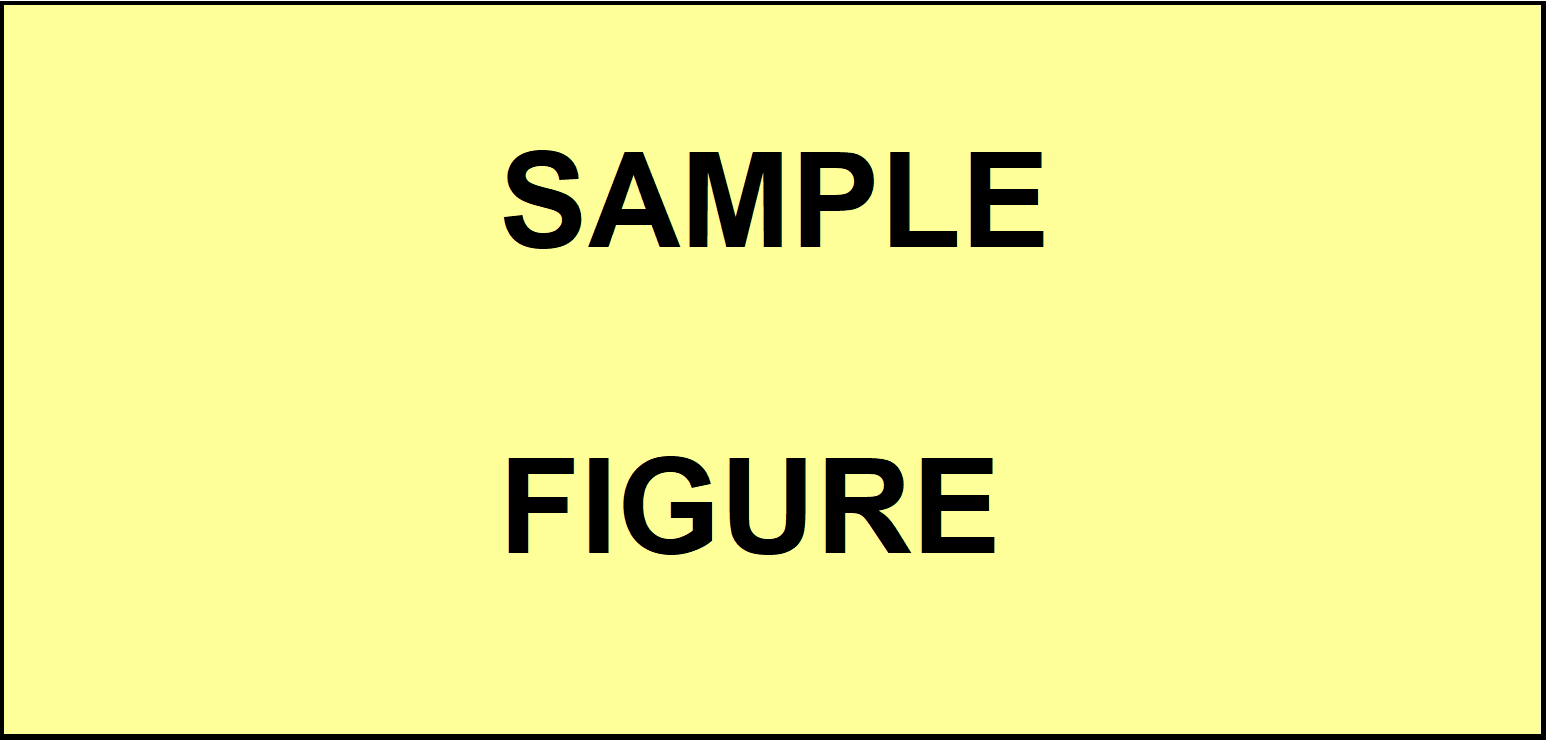
\includegraphics[width=290pt,keepaspectratio=true]{./fig/sekil4}
 % sekil4.eps: 0x0 pixel, 300dpi, 0.00x0.00 cm, bb=14 14 1148 603
 \caption{Figure captions must be ended with a full stop.}
 \label{fig:ch3-3}
\end{figure}
\vspace{-9pt} % 12pt 

Lorem ipsum dolor sit amet, consetetur sadipscing elitr, sed diam nonumy eirmod tempor invidunt ut labore et dolore magna aliquyam erat, sed diam voluptua. At vero eos et accusam et justo duo dolores et ea rebum. Stet clita kasd gub rgren, no sea takimata sanctus est Lorem ipsum dolor sit amet, consetetur sadipscing elitr, sed diam nonumy eirmod tempor invidunt ut lab ore sit et dolore magna (3.2). Lorem ipsum dolor sit amet, consetetur sadipscing elitr, sed diam nonumy eirmod tempor invidunt ut labore et dolore magna aliquyam erat, sed diam voluptua. At vero eos et accusam et justo duo dolores et ea rebum. Lorem ipsum dolor sit amet, consetetur sadipscing elitr, sed diam nonumy eirmod tempor invidunt ut labore et dolore magna aliquyam erat, sed diam voluptua. At vero eos et accusam et justo duo dolores et ea rebum. Lorem ipsum dolor sit amet, consetetur sadipscing elitr, sed diam nonumy eirmod tempor invidunt ut labore et dolore magna aliquyam erat, sed diam voluptua. At vero eos et accusam et justo duo dolores et ea rebum Equation \eqref{eq:ch3-2}.
%
\begin{equation}\label{eq:ch3-2}
	D\left(C_{A},C_{B}\right) = \min X_{A}\in C_{A},X_{B}\in C_{B} 
     d\left(X_{A},X_{B}\right)
\end{equation}
%
Lorem ipsum dolor sit amet, consetetur sadipscing elitr, sed diam nonumy eirmod tempor invidunt ut labore et dolore magna aliquyam erat, sed diam voluptua. Lorem ipsum dolor sit amet, consetetur sadipscing elitr, sed diam nonumy eirmod tempor invidunt ut labore et dolore magna aliquyam erat, sed diam voluptua. At vero eos et accusam et justo duo dolores et ea rebum.

\section{Practical Applications}

Lorem ipsum dolor sit amet, consetetur sadipscing elitr, sed diam nonumy eirmod tempor invidunt ut labore et dolore magna aliquyam erat, sed diam voluptua. At vero eos et accusam et justo duo dolores et ea rebum. Stet clita kasd gub rgren, no sea takimata sanctus est Lorem ipsum dolor sit amet, consetetur sadipscing elitr, sed diam nonumy eirmod tempor invidunt ut lab ore sit et dolore magna.

Lorem ipsum dolor sit amet, consetetur sadipscing elitr, sed diam nonumy eirmod tempor invidunt ut labore et dolore magna aliquyam erat, sed diam voluptua. At vero eos et accusam et justo duo dolores et ea rebum. Stet clita kasd gub rgren, no sea takimata sanctus est Lorem ipsum dolor sit amet, consetetur sadipscing elitr, sed diam nonumy eirmod tempor invidunt ut lab ore sit et dolore magna.

\section{Application Data}

Lorem ipsum dolor sit amet, consetetur sadipscing elitr, sed diam nonumy eirmod tempor invidunt ut labore et dolore magna aliquyam erat, sed diam voluptua. At vero eos et accusam et justo duo dolores et ea rebum. Stet clita kasd gub rgren, no sea takimata sanctus est Lorem ipsum dolor sit amet, consetetur sadipscing elitr, sed diam nonumy eirmod tempor invidunt ut lab ore sit et dolore magna.

Lorem ipsum dolor sit amet, consetetur sadipscing elitr, sed diam nonumy eirmod tempor invidunt ut labore et dolore magna aliquyam erat, sed diam voluptua. At vero eos et accusam et justo duo dolores et ea rebum. Lorem ipsum dolor sit amet, consetetur sadipscing elitr, sed diam nonumy eirmod tempor invidunt ut labore et dolore magna aliquyam erat, sed diam voluptua.

%%%%%%%%%%%%%%%%%%%%%%%%%%%%%%%%%%%%%%%%%%%%%%%%%%%%%%%%%%%%%%%%%
\chapter{REFERENCES, QUOTINGS AND FOOTNOTES}\label{ch:ch4}
%%%%%%%%%%%%%%%%%%%%%%%%%%%%%%%%%%%%%%%%%%%%%%%%%%%%%%%%%%%%%%%%%

In this section, information will be given about how citations, quotings and footnotes should be.

\section{Citing (indication of references in main text body)}

\vspace{-12pt}

\subsection{Citing according to surname of author}

References are cited with the surname of author and year. In the references section, the references are listed alphabetically according to the surname of the author \citep{acar97}.

Citing of a reference at the beginning of or within a sentence must be as \citet{harper2007}, whereas a citation at the end of a sentence must be as (Boran, 2003). The full-stop is placed directly after the citation. 

A reference with two authors must be cited as \citeauthor{mccaffrey88} (\citeyear{mccaffrey88}) at the beginning of or within a sentence, or as (\citeauthor{mccaffrey88}, \citeyear{mccaffrey88}) at the end of a sentence. 

A reference with more than two authors must be cited as \citeauthor{vanden2001} (\citeyear{vanden2001}) at the beginning of or within a sentence, or as (\citeauthor{vanden2001}, \citeyear{vanden2001}) at the end of a sentence. 

Different publications of an author published in the same year must be cited as Feray (2005a), Feray (2005b).

While citing a part of a publication; the number of the page the cited material (chapter, table, figure, or equation) is on must be indicated. While citing, the expression “page” must be abbreviated, but “chapter” must not. For example; (Centers for Disease Control and Prevention, 2005, p. 10), (Shimamura, 1989, Chapter 3). 

Citing multiple publications in one pair of brackets; (Berndt, 2002; Harlow, 1983) 

Citing personal communication in main text body; (V.–G. Nguyen, personal communication, September 28, 1998), (J. Smith, personal communication, August 15, 2009).

In the references section, reference tags must be listed according to the surname of author. 

For citing of secondary references (In case the reference cites another reference), the secondary reference must be cited in brackets.  In the references section, the reference tag is organized according to the secondary reference, the original reference must not be used as a tag. For example; In his e-mails, Smith argued that asynchronous line dancing would be the next Internet meme (as cited in Jones, 2010).

\subsubsection{Citing according to order of appearance}

References are cited by numbering and indicating the number in square brackets ([]) in the main text body. The first reference cited in a thesis is numbered [1] and the following references are numbered according to the order of appearance.

In the main text body, references must be cited as specified below:

[1]	Reference no. 1

[1-3]	References from no.1 to 3 (thus, references 1,2 and 3)

[1,3]	References no. 1 and 3

[1,3,8]	References no.1, 3 and 8

[1,3-8]	References no.1, and from no.3 to 8 (thus, references 1, 3, 4, 5, 6, 7 and 8)

Different volumes of a reference must be cited and numbered individually.

Cite command examples are:

\begin{itemize}
    \item \cite{sisaky}
    \item \citep{sisaky}
    \item \citet{sisaky}
    \item \citet*{sisaky}
    \item (\citeauthor{sisaky} (\citeyear{sisaky}) \citep{sisaky})
    \item (\citeauthor*{sisaky} (\citeyear{sisaky}) \citep{sisaky})
    \item \citet[\chaptername\ \ref{ch:ch4}]{sisaky} 
  \end{itemize}

\vfill\phantom{.}\\

Multiple citation examples are:

\begin{itemize}
    \item \cite{Burke74,17590413,Wegener2000629}
    \item \citep{Burke74,17590413,Wegener2000629}
    \item \citet{Burke74,17590413,Wegener2000629}
    \item \citep*{Burke74,17590413,Wegener2000629}
    \item \citet*{Burke74,17590413,Wegener2000629}
  \end{itemize}

\section{Quoting}

Generally, quoting is done by remaining faithful to the original text in terms of words, spelling and punctuation. In case there is a mistake, the correct version is written in square brackets in the quoted text.

Short quotations (not longer than 40 words) must be given in quotation marks. Following the text quoted, the reference must be written and a full-stop must be placed afterwards.  

Quotations longer than 40 words must not be shown in quotation  marks. Instead, they must be indented 1 tab space (1.27 cm) from the left side of the page. The font size for long quotations indented from the left must be 2 pt smaller than the font size used in main text body. However, it is not advised to quote very long texts and to quote very frequently. Unlike short quotations, references of long quotations must be placed after the full stop. (i.e., .(p.196))

Example for a quotation at the beginning of a sentence;

According to Jones (1998), "Students often had difficulty using APA style,  especially when it was their first time" (p. 199).

Example for a quotation in the middle of a sentence;

Interpreting these results, Robbins et al. (2003) suggested that the “therapists in dropout cases may have inadvertently validated parental negativity about the adolescent without adequately responding to the adolescent’s needs or concerns” (p. 541) contributing to an overall climate of negativity.

Example for a quotation at the end of a sentence;

Confusing this issue is the overlapping nature of roles in palliative care, whereby “medical needs are met by those in the medical disciplines; nonmedical needs may be addressed by anyone on the team” (Csikai \& Chaitin, 2006, p. 112). 

Detailed information on quoting could be found on websites of Graduate Schools and associated links.

\section{Footnotes}

Footnotes could be used in theses to add content-expanding, content-enhancing, or additional information\footnote{Reference display can not be done with footnotes. Footnotes could be used in theses to add content-expanding, content-enhancing, or additional information. If these informations must include references, these references must be indicated in References section.}. 

Footnote numbers must be placed directly after a quotation. In case the quotation is a paragraph, the footnote numbers must be placed directly after the last word of the paragraph (as superscript). In case the quotation is a concept or a noun, footnote numbers must be placed directly after that concept or noun (as superscript). 

Footnote numbers in the main text body must be indicated as subscript\footnote{Footnotes must be written with a font size 2 pt smaller than the main text body font size.}, as shown. A punctuation mark must not be placed after the number.

Footnotes must be written with a font size 2 pt smaller than the main text body font size. 

1 space must be set between footnote line and footnote number, 1/2 space must be set between footnote number and the first line of the footnote. Footnotes must be separated from the main text body with a thin horizontal line. 

Detailed information on footnotes could be found on the websites of Graduate Schools and associated links.

\section{Second Level Title: First Letters Capital}

Lorem ipsum dolor sit amet, consetetur sadipscing elitr, sed diam nonumy eirmod tempor invidunt ut labore et dolore magna aliquyam erat, sed diam voluptua. At vero eos et accusam et justo duo dolores et ea rebum. Stet clita kasd gub rgren, no sea \citep{Zuckerman199486}.

\subsection{Third level title: Only first letter capital}

\citet{Wolchik2000843} Lorem ipsum dolor sit amet, consetetur sadipscing elitr, sed diam nonumy eirmod tempor invidunt ut labore et dolore magna aliquyam erat, sed diam voluptua. At vero eos et accusam et justo duo dolores et ea rebum. Stet clita kasd gub rgren, no sea 

\subsubsection{Fourth level title: Only first letter capital}

\citet{Box:1990:TSA:574978} Stet clita kasd gub rgren, no sea takimata sanctus est Lorem ipsum dolor sit amet, consetetur sadipscing elitr, sed diam nonumy eirmod tempor invidunt ut lab ore sit et dolore magna \citep{HYP:HYP57}.

\subsubsubsection{Fifth level title: Only first letter capital}

Stet clita kasd gub rgren, no sea takimata sanctus est Lorem ipsum dolor sit amet, consetetur sadipscing elitr, sed diam nonumy eirmod tempor invidunt ut lab ore sit et dolore magna \citep{url-1,url-2}.

\vspace{6pt} % 12pt
\begin{figure}[!ht]
 \centering
 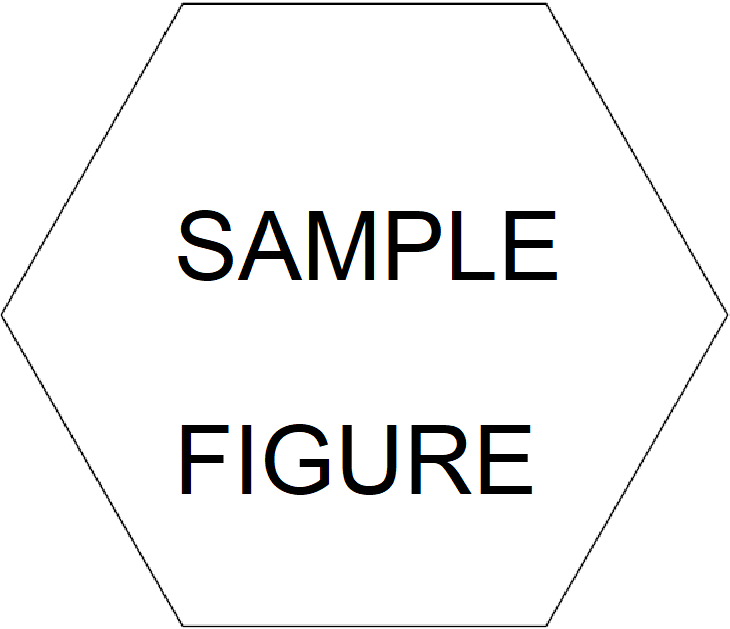
\includegraphics[width=230pt,keepaspectratio=true]{./fig/sekil6.png}
 % sekil6.eps: 0x0 pixel, 300dpi, 0.00x0.00 cm, bb=14 14 555 489
 \caption{For a multi-line figure captions, it is important that all the
  lines of the caption are aligned.}
 \label{fig:ch4-1}
\end{figure}
\vspace{-9pt} % 12pt 

\cite{TS-40561} Stet clita kasd gub rgren, no sea takimata sanctus est Lorem ipsum dolor sit amet, consetetur sadipscing elitr, sed diam nonumy eirmod tempor invidunt ut lab ore sit et dolore magna. Stet clita kasd gub rgren, no sea takimata sanctus est Lorem ipsum dolor sit amet, consetetur sadipscing elitr, sed diam nonumy eirmod tempor invidunt ut lab ore sit et dolore magna \cite{startrek,simpsondvd}. 

\citet{nelson88,moore91} Stet clita kasd gub rgren, no sea takimata sanctus est Lorem ipsum dolor sit amet, consetetur sadipscing elitr, sed diam nonumy eirmod tempor invidunt ut lab ore sit et dolore magna \citep{unesco}. 

\vspace{6pt} % 12pt
\begin{table}[!ht]
\centering
\setlength{\tabcolsep}{14pt}
\caption{Example table.}
\begin{tabular}{cccc}
\toprule\midrule
Column A & Column B & Column C & Column D \\
\midrule
Row A & Row A & Row A & Row A \\
Row B & Row B & Row B & Row B \\
Row C & Row C & Row C & Row C \\
\bottomrule
\end{tabular}
\label{table:ch4-1}
\end{table}
\vspace{-9pt} % 12pt 

Lorem ipsum dolor sit amet, consectetur adipiscing elit. Sed ac augue vel dui  adipiscing placerat et nec metus. Donec bibendum sodales mollis. Cras in lacus  justo, at vestibulum quam. Sed semper, est sit amet consectetur ornare, leo est  lacinia velit, adipiscing elementum lectus felis at sem. Aenean hendrerit erat eu  lacus malesuada at sodales arcu egestas. Maecenas euismod urna ut sem luctus et  congue metus vulputate. Ut pellentesque, neque eget fringilla elementum, ligula  massa aliquet lorem, et varius nisi lacus vel diam. Etiam vitae metus sed orci  rutrum fringilla. Phasellus sed velit quam. Mauris vestibulum, mauris a cursus  adipiscing, nulla est hendrerit justo, ut fringilla eros velit ut mauris.
%%%%%%%%%%%%%%%%%%%%%%%%%%%%%%%%%%%%%%%%%%%%%%%%%%%%%%%%%%%%%%%%%
\chapter{(IF NECESSARY) CHAPTER 5}\label{ch:ifnecch5}
%%%%%%%%%%%%%%%%%%%%%%%%%%%%%%%%%%%%%%%%%%%%%%%%%%%%%%%%%%%%%%%%%

Lorem ipsum dolor sit amet, consetetur sadipscing elitr, sed diam nonumy eirmod tempor invidunt ut labore et dolore magna aliquyam erat, sed diam voluptua. At vero eos et accusam et justo duo dolores et ea rebum. Stet clita kasd gub rgren, no sea takimata sanctus est Lorem ipsum dolor sit amet, consetetur sadipscing elitr, sed diam nonumy eirmod tempor invidunt ut lab ore sit et dolore magna.

\section{Practical Application of This Study}

In this thesis, the necessary steps for constructing an end-to-end streamflow forecasting system were discussed. These steps include the use 

\section{Second Level Title: First Letters Capital}

Lorem ipsum dolor sit amet, consetetur sadipscing elitr, sed diam nonumy eirmod tempor invidunt ut labore et dolore magna aliquyam erat, sed diam voluptua. At vero eos et accusam et justo duo dolores et ea rebum. Stet clita kasd gub rgren, no sea 

\subsection{Third level title: Only first letter capital}

Lorem ipsum dolor sit amet, consetetur sadipscing elitr, sed diam nonumy eirmod tempor invidunt ut labore et dolore magna aliquyam erat, sed diam voluptua. At vero eos et accusam et justo duo dolores et ea rebum. Stet clita kasd gub rgren, no sea 

\subsubsection{Fourth level title: Only first letter capital}

Stet clita kasd gub rgren, no sea takimata sanctus est Lorem ipsum dolor sit amet, consetetur sadipscing elitr, sed diam nonumy eirmod tempor invidunt ut lab ore sit et dolore magna. 

\subsubsubsection{Fifth level title: No numbering after fourth level titles}

Lorem ipsum dolor sit amet, consetetur sadipscing elitr, sed diam nonumy eirmod tempor invidunt ut labore et dolore magna aliquyam erat, sed diam voluptua Figure \ref{fig:ch5-1}. This indicates that the ANN is accurate at base flow and flow height values lower then 3 m. 

\vspace{6pt} % 12pt
\begin{figure}[!ht]
    \centering
    
\includegraphics[width=230pt,keepaspectratio=true]{./fig/sekil5}
    % sekil5.eps: 0x0 pixel, 300dpi, 0.00x0.00 cm, bb=14 14 1193 701
    \caption{For a multi-line figure captions, it is important that all the
    lines of the caption are aligned.}
    \label{fig:ch5-1}
\end{figure}
\vspace{-9pt} % 12pt 

Stet clita kasd gub rgren, no sea takimata sanctus est Lorem ipsum dolor sit amet, consetetur sadipscing elitr, sed diam nonumy eirmod tempor invidunt ut lab ore sit et dolore magna. Stet clita kasd gub rgren, no sea takimata sanctus est Lorem ipsum dolor sit amet, consetetur sadipscing elitr, sed diam nonumy eirmod tempor invidunt ut lab ore sit et dolore magna Table \ref{table:ch5-1}.

\vspace{6pt} % 12pt
\begin{table}[!ht]
\centering
\setlength{\tabcolsep}{14pt}
\caption{Example table in chapter 5.}
\begin{tabular}{cccc}
\toprule\midrule
Column A & Column B & Column C & Column D \\
\midrule
Row A & Row A & Row A & Row A \\
Row B & Row B & Row B & Row B \\
Row C & Row C & Row C & Row C \\
\bottomrule
\end{tabular}
\label{table:ch5-1}
\end{table}
\vspace{-9pt} % 12pt 

Stet clita kasd gub rgren, no sea takimata sanctus est Lorem ipsum dolor sit amet, consetetur sadipscing elitr, sed diam nonumy eirmod tempor invidunt ut lab ore sit et dolore magna. Stet clita kasd gub rgren, no sea takimata sanctus est Lorem ipsum dolor sit amet, consetetur sadipscing elitr, sed diam nonumy eirmod tempor invidunt ut lab ore sit et dolore magna. 

Lorem ipsum dolor sit amet, consectetur adipiscing elit. Sed ac augue vel dui  adipiscing placerat et nec metus. Donec bibendum sodales mollis. Cras in lacus  justo, at vestibulum quam. Sed semper, est sit amet consectetur ornare, leo est  lacinia velit, adipiscing elementum lectus felis at sem. Aenean hendrerit erat eu  lacus malesuada at sodales arcu egestas. Maecenas euismod urna ut sem luctus et  congue metus vulputate. Ut pellentesque, neque eget fringilla elementum, ligula  massa aliquet lorem, et varius nisi lacus vel diam. Etiam vitae metus sed orci  rutrum fringilla. Phasellus sed velit quam. Mauris vestibulum, mauris a cursus  adipiscing, nulla est hendrerit justo, ut fringilla eros velit ut mauris.
%%%%%%%%%%%%%%%%%%%%%%%%%%%%%%%%%%%%%%%%%%%%%%%%%%%%%%%%%%%%%%%%%
\chapter{CONCLUSIONS AND RECOMMENDATIONS }\label{ch:ch6}
%%%%%%%%%%%%%%%%%%%%%%%%%%%%%%%%%%%%%%%%%%%%%%%%%%%%%%%%%%%%%%%%%

Lorem ipsum dolor sit amet, consetetur sadipscing elitr, sed diam nonumy eirmod tempor invidunt ut labore et dolore magna aliquyam erat, sed diam voluptua. At vero eos et accusam et justo duo dolores et ea rebum. Stet clita kasd gub rgren, no sea takimata sanctus est Lorem ipsum dolor sit amet, consetetur sadipscing elitr, sed diam nonumy eirmod tempor invidunt ut lab ore sit et dolore magna.

\section{Practical Application of This Study}

Lorem ipsum dolor sit amet, consetetur sadipscing elitr, sed diam nonumy eirmod tempor invidunt ut labore et dolore magna aliquyam erat, sed diam voluptua. At vero eos et accusam et justo duo dolores et ea rebum. Stet clita kasd gub rgren, no sea takimata sanctus est Lorem ipsum dolor sit amet, consetetur sadipscing elitr, sed diam nonumy eirmod tempor invidunt ut lab ore sit et dolore magna.

\section{Second Level Title: First Letters Capital}

Lorem ipsum dolor sit amet, consetetur sadipscing elitr, sed diam nonumy eirmod tempor invidunt ut labore et dolore magna aliquyam erat, sed diam voluptua. At vero eos et accusam et justo duo dolores et ea rebum. Stet clita kasd gub rgren, no sea 

\subsection{Third level title: Only first letter capital}

Lorem ipsum dolor sit amet, consetetur sadipscing elitr, sed diam nonumy eirmod tempor invidunt ut labore et dolore magna aliquyam erat, sed diam voluptua. At vero eos et accusam et justo duo dolores et ea rebum. Stet clita kasd gub rgren, no sea 

\subsubsection{Fourth level title: Only first letter capital}

Stet clita kasd gub rgren, no sea takimata sanctus est Lorem ipsum dolor sit amet, consetetur sadipscing elitr, sed diam nonumy eirmod tempor invidunt ut lab ore sit et dolore magna. 

\textbf{Fifth level title: no numbering after fourth level titles}

Stet clita kasd gub rgren, no sea takimata sanctus est Lorem ipsum dolor sit amet, consetetur sadipscing elitr, sed diam nonumy eirmod tempor invidunt ut lab ore sit et dolore magna. 

\vspace{6pt} % 12pt
\begin{figure}[!ht]
    \centering
    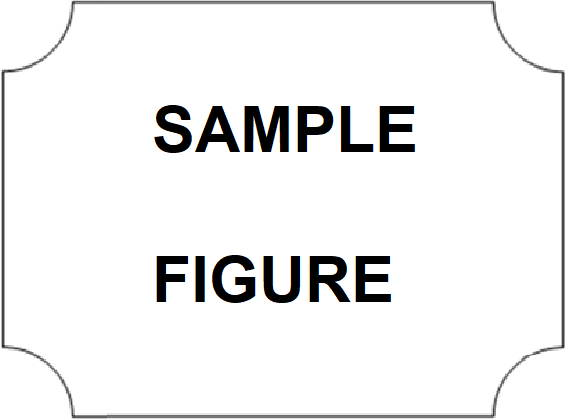
\includegraphics[width=230pt,keepaspectratio=true]{./fig/sekil7}
    % sekil7.eps: 0x0 pixel, 300dpi, 0.00x0.00 cm, bb=14 14 455 369
    \caption{Example figure in chapter 6.}
    \label{fig:ch6-1}
\end{figure}
\vspace{-6pt} % 12pt 

Stet clita kasd gub rgren, no sea takimata sanctus est Lorem ipsum dolor sit amet, consetetur sadipscing elitr, sed diam nonumy eirmod tempor invidunt ut lab ore sit et dolore magna. Stet clita kasd gub rgren, no sea takimata sanctus est Lorem ipsum dolor sit amet, consetetur sadipscing elitr, sed diam nonumy eirmod tempor invidunt ut lab ore sit et dolore magna. Stet clita kasd gub rgren, no sea takimata sanctus est Lorem ipsum dolor sit amet, consetetur sadipscing elitr, sed diam nonumy eirmod tempor invidunt ut lab ore sit et dolore magna. 
Stet clita kasd gub rgren, no sea takimata sanctus est Lorem ipsum dolor sit amet, consetetur sadipscing elitr, sed diam nonumy eirmod tempor invidunt ut lab ore sit et dolore magna. 

\vspace{6pt} % 12pt
\begin{table}[!ht]
\centering
\setlength{\tabcolsep}{14pt}
\caption{Example table in chapter 6.}
\label{table:ch6-1}
\begin{tabular}{cccc}
\toprule\midrule
Column A & Column B & Column C & Column D \\
\midrule
Row A & Row A & Row A & Row A \\
Row B & Row B & Row B & Row B \\
Row C & Row C & Row C & Row C \\
\bottomrule
\end{tabular}
\end{table}
\vspace{-6pt} % 12pt 

Lorem ipsum dolor sit amet, consectetur adipiscing elit. Sed ac augue vel dui  adipiscing placerat et nec metus. Donec bibendum sodales mollis. Cras in lacus   justo, at vestibulum quam. Sed semper, est sit amet consectetur ornare, leo est  lacinia velit, adipiscing elementum lectus felis at sem. Aenean hendrerit erat eu  lacus malesuada at sodales arcu egestas. Maecenas euismod urna ut sem luctus et  congue metus vulputate. Ut pellentesque, neque eget fringilla elementum, ligula  massa aliquet lorem, et varius nisi lacus vel diam. Etiam vitae metus sed orci  rutrum fringilla. Phasellus sed velit quam. Mauris vestibulum, mauris a cursus  adipiscing, nulla est hendrerit justo, ut fringilla eros velit ut mauris.

% ---------------------------------------------------------------- %
% Form tez.bib to contain your references in bibtex format         %
% use \citet, \citep, \cite commands for citing your references    %
% ---------------------------------------------------------------- %
\bibliographystyle{itubib_num}        
\bibliography{tez}

% ---------------------------------------------------------------- %
% Experimental aurhor year bibliography style                      %
% use \citet, \citep, \cite commands for citing your references    %
% ---------------------------------------------------------------- %
%\bibliographystyle{itubib_name}        
%\bibliography{tez}

% ---------------------------------------------------------------- %
% Appendix files. EklerKapak is the appendix title page.           %
% ---------------------------------------------------------------- %
\EklerKapak

\textbf{APPENDIX A :} Maps\\
\textbf{APPENDIX B :} Other Maps\\


% ---------------------------------------------------------------- %
% \EklerBolum forms and appendix of  chapters.                     %
% ---------------------------------------------------------------- %
\EklerBolum

\chapter{Maps}

Lorem ipsum dolor sit amet, consectetur adipiscing elit. Sed ac augue vel dui  adipiscing placerat et nec metus. Donec bibendum sodales mollis. Cras in lacus  justo, at vestibulum quam. Sed semper, est sit amet consectetur ornare, leo est  lacinia velit, adipiscing elementum lectus felis at sem.

Lorem ipsum dolor sit amet, consectetur adipiscing elit. Sed ac augue vel dui  adipiscing placerat et nec metus. Donec bibendum sodales mollis. Cras in lacus  justo, at vestibulum quam. Sed semper, est sit amet consectetur ornare, leo est  lacinia velit, adipiscing elementum lectus felis at sem.

\begin{table}[!ht]
\centering
\setlength{\tabcolsep}{14pt}
\caption{Example table in appendix.}
\begin{tabular}{cccc}
\toprule\midrule
Column A & Column B & Column C & Column D \\
\hline
Row A & Row A & Row A & Row A \\
Row B & Row B & Row B & Row B \\
Row C & Row C & Row C & Row C \\
\bottomrule
\end{tabular}
\label{table:appendix}
\end{table}

Lorem ipsum dolor sitamet, consectetur adipiscing elit. Sed ac augue vel dui  adipiscing placerat et nec metus. Donec bibendum sodales mollis. Cras in lacus  justo, at vestibulum quam. Sed semper, est sit amet consectetur ornare, leo est  lacinia velit, adipiscing elementum lectus felis at sem.

\chapter{Other Maps}

Lorem ipsum dolor sit amet, consectetur adipiscing elit. Sed ac augue vel dui  adipiscing placerat et nec metus. Donec bibendum sodales mollis. Cras in lacus  justo, at vestibulum quam. Sed semper, est sit amet consectetur ornare, leo est  lacinia velit, adipiscing elementum lectus felis at sem.
%
\begin{equation}
    y_{t} = \phi_{1} y_{t-1} + \epsilon_{t}
\label{eq:appendix}
\end{equation}
%
Lorem ipsum dolor sit amet, consectetur adipiscing elit. Sed ac augue vel dui  adipiscing placerat et nec metus. Donec bibendum sodales mollis. Cras in lacus  justo, at vestibulum quam. Sed semper, est sit amet consectetur ornare, leo est  lacinia velit, adipiscing elementum lectus felis at sem.

\begin{figure}[!ht]
    \centering
    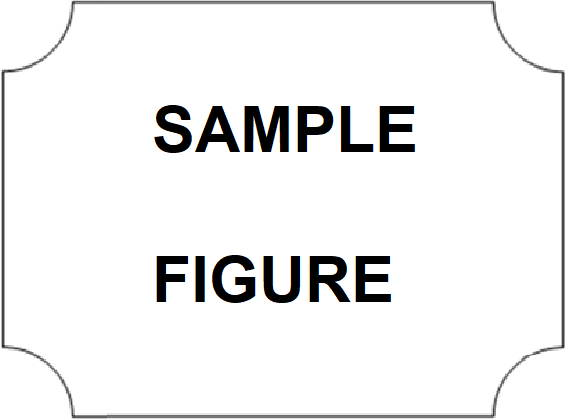
\includegraphics[width=230pt,keepaspectratio=true]{./fig/sekil7}
    % sekil7.eps: 0x0 pixel, 300dpi, 0.00x0.00 cm, bb=14 14 455 369
    \caption{Example figure in appendix.}
    \label{fig:appendix}
\end{figure}

Lorem ipsum dolor sit amet, consectetur adipiscing elit. Sed ac augue vel dui  adipiscing placerat et nec metus. Donec bibendum sodales mollis. Cras in lacus  justo, at vestibulum quam. Sed semper, est sit amet consectetur ornare, leo est  lacinia velit, adipiscing elementum lectus felis at sem.






% ---------------------------------------------------------------- %
% The resume page                                                 %
% ---------------------------------------------------------------- %

\OzgecmisPage
\SirtPage

% ---------------------------------------------------------------- %
% The document ends                                                 %
% ---------------------------------------------------------------- %


\end{document}                      

% ---------------------------------------------------------------- %
% About this template: iletisim@be.itu.edu.tr                      %
% ---------------------------------------------------------------- %
